\documentclass[11pt]{article}

    \usepackage[breakable]{tcolorbox}
    \usepackage{parskip} % Stop auto-indenting (to mimic markdown behaviour)
    

    % Basic figure setup, for now with no caption control since it's done
    % automatically by Pandoc (which extracts ![](path) syntax from Markdown).
    \usepackage{graphicx}
    % Keep aspect ratio if custom image width or height is specified
    \setkeys{Gin}{keepaspectratio}
    % Maintain compatibility with old templates. Remove in nbconvert 6.0
    \let\Oldincludegraphics\includegraphics
    % Ensure that by default, figures have no caption (until we provide a
    % proper Figure object with a Caption API and a way to capture that
    % in the conversion process - todo).
    \usepackage{caption}
    \DeclareCaptionFormat{nocaption}{}
    \captionsetup{format=nocaption,aboveskip=0pt,belowskip=0pt}

    \usepackage{float}
    \floatplacement{figure}{H} % forces figures to be placed at the correct location
    \usepackage{xcolor} % Allow colors to be defined
    \usepackage{enumerate} % Needed for markdown enumerations to work
    \usepackage{geometry} % Used to adjust the document margins
    \usepackage{amsmath} % Equations
    \usepackage{amssymb} % Equations
    \usepackage{textcomp} % defines textquotesingle
    % Hack from http://tex.stackexchange.com/a/47451/13684:
    \AtBeginDocument{%
        \def\PYZsq{\textquotesingle}% Upright quotes in Pygmentized code
    }
    \usepackage{upquote} % Upright quotes for verbatim code
    \usepackage{eurosym} % defines \euro

    \usepackage{iftex}
    \ifPDFTeX
        \usepackage[T1]{fontenc}
        \IfFileExists{alphabeta.sty}{
              \usepackage{alphabeta}
          }{
              \usepackage[mathletters]{ucs}
              \usepackage[utf8x]{inputenc}
          }
    \else
        \usepackage{fontspec}
        \usepackage{unicode-math}
    \fi

    \usepackage{fancyvrb} % verbatim replacement that allows latex
    \usepackage{grffile} % extends the file name processing of package graphics
                         % to support a larger range
    \makeatletter % fix for old versions of grffile with XeLaTeX
    \@ifpackagelater{grffile}{2019/11/01}
    {
      % Do nothing on new versions
    }
    {
      \def\Gread@@xetex#1{%
        \IfFileExists{"\Gin@base".bb}%
        {\Gread@eps{\Gin@base.bb}}%
        {\Gread@@xetex@aux#1}%
      }
    }
    \makeatother
    \usepackage[Export]{adjustbox} % Used to constrain images to a maximum size
    \adjustboxset{max size={0.9\linewidth}{0.9\paperheight}}

    % The hyperref package gives us a pdf with properly built
    % internal navigation ('pdf bookmarks' for the table of contents,
    % internal cross-reference links, web links for URLs, etc.)
    \usepackage{hyperref}
    % The default LaTeX title has an obnoxious amount of whitespace. By default,
    % titling removes some of it. It also provides customization options.
    \usepackage{titling}
    \usepackage{longtable} % longtable support required by pandoc >1.10
    \usepackage{booktabs}  % table support for pandoc > 1.12.2
    \usepackage{array}     % table support for pandoc >= 2.11.3
    \usepackage{calc}      % table minipage width calculation for pandoc >= 2.11.1
    \usepackage[inline]{enumitem} % IRkernel/repr support (it uses the enumerate* environment)
    \usepackage[normalem]{ulem} % ulem is needed to support strikethroughs (\sout)
                                % normalem makes italics be italics, not underlines
    \usepackage{soul}      % strikethrough (\st) support for pandoc >= 3.0.0
    \usepackage{mathrsfs}
    

    
    % Colors for the hyperref package
    \definecolor{urlcolor}{rgb}{0,.145,.698}
    \definecolor{linkcolor}{rgb}{.71,0.21,0.01}
    \definecolor{citecolor}{rgb}{.12,.54,.11}

    % ANSI colors
    \definecolor{ansi-black}{HTML}{3E424D}
    \definecolor{ansi-black-intense}{HTML}{282C36}
    \definecolor{ansi-red}{HTML}{E75C58}
    \definecolor{ansi-red-intense}{HTML}{B22B31}
    \definecolor{ansi-green}{HTML}{00A250}
    \definecolor{ansi-green-intense}{HTML}{007427}
    \definecolor{ansi-yellow}{HTML}{DDB62B}
    \definecolor{ansi-yellow-intense}{HTML}{B27D12}
    \definecolor{ansi-blue}{HTML}{208FFB}
    \definecolor{ansi-blue-intense}{HTML}{0065CA}
    \definecolor{ansi-magenta}{HTML}{D160C4}
    \definecolor{ansi-magenta-intense}{HTML}{A03196}
    \definecolor{ansi-cyan}{HTML}{60C6C8}
    \definecolor{ansi-cyan-intense}{HTML}{258F8F}
    \definecolor{ansi-white}{HTML}{C5C1B4}
    \definecolor{ansi-white-intense}{HTML}{A1A6B2}
    \definecolor{ansi-default-inverse-fg}{HTML}{FFFFFF}
    \definecolor{ansi-default-inverse-bg}{HTML}{000000}

    % common color for the border for error outputs.
    \definecolor{outerrorbackground}{HTML}{FFDFDF}

    % commands and environments needed by pandoc snippets
    % extracted from the output of `pandoc -s`
    \providecommand{\tightlist}{%
      \setlength{\itemsep}{0pt}\setlength{\parskip}{0pt}}
    \DefineVerbatimEnvironment{Highlighting}{Verbatim}{commandchars=\\\{\}}
    % Add ',fontsize=\small' for more characters per line
    \newenvironment{Shaded}{}{}
    \newcommand{\KeywordTok}[1]{\textcolor[rgb]{0.00,0.44,0.13}{\textbf{{#1}}}}
    \newcommand{\DataTypeTok}[1]{\textcolor[rgb]{0.56,0.13,0.00}{{#1}}}
    \newcommand{\DecValTok}[1]{\textcolor[rgb]{0.25,0.63,0.44}{{#1}}}
    \newcommand{\BaseNTok}[1]{\textcolor[rgb]{0.25,0.63,0.44}{{#1}}}
    \newcommand{\FloatTok}[1]{\textcolor[rgb]{0.25,0.63,0.44}{{#1}}}
    \newcommand{\CharTok}[1]{\textcolor[rgb]{0.25,0.44,0.63}{{#1}}}
    \newcommand{\StringTok}[1]{\textcolor[rgb]{0.25,0.44,0.63}{{#1}}}
    \newcommand{\CommentTok}[1]{\textcolor[rgb]{0.38,0.63,0.69}{\textit{{#1}}}}
    \newcommand{\OtherTok}[1]{\textcolor[rgb]{0.00,0.44,0.13}{{#1}}}
    \newcommand{\AlertTok}[1]{\textcolor[rgb]{1.00,0.00,0.00}{\textbf{{#1}}}}
    \newcommand{\FunctionTok}[1]{\textcolor[rgb]{0.02,0.16,0.49}{{#1}}}
    \newcommand{\RegionMarkerTok}[1]{{#1}}
    \newcommand{\ErrorTok}[1]{\textcolor[rgb]{1.00,0.00,0.00}{\textbf{{#1}}}}
    \newcommand{\NormalTok}[1]{{#1}}

    % Additional commands for more recent versions of Pandoc
    \newcommand{\ConstantTok}[1]{\textcolor[rgb]{0.53,0.00,0.00}{{#1}}}
    \newcommand{\SpecialCharTok}[1]{\textcolor[rgb]{0.25,0.44,0.63}{{#1}}}
    \newcommand{\VerbatimStringTok}[1]{\textcolor[rgb]{0.25,0.44,0.63}{{#1}}}
    \newcommand{\SpecialStringTok}[1]{\textcolor[rgb]{0.73,0.40,0.53}{{#1}}}
    \newcommand{\ImportTok}[1]{{#1}}
    \newcommand{\DocumentationTok}[1]{\textcolor[rgb]{0.73,0.13,0.13}{\textit{{#1}}}}
    \newcommand{\AnnotationTok}[1]{\textcolor[rgb]{0.38,0.63,0.69}{\textbf{\textit{{#1}}}}}
    \newcommand{\CommentVarTok}[1]{\textcolor[rgb]{0.38,0.63,0.69}{\textbf{\textit{{#1}}}}}
    \newcommand{\VariableTok}[1]{\textcolor[rgb]{0.10,0.09,0.49}{{#1}}}
    \newcommand{\ControlFlowTok}[1]{\textcolor[rgb]{0.00,0.44,0.13}{\textbf{{#1}}}}
    \newcommand{\OperatorTok}[1]{\textcolor[rgb]{0.40,0.40,0.40}{{#1}}}
    \newcommand{\BuiltInTok}[1]{{#1}}
    \newcommand{\ExtensionTok}[1]{{#1}}
    \newcommand{\PreprocessorTok}[1]{\textcolor[rgb]{0.74,0.48,0.00}{{#1}}}
    \newcommand{\AttributeTok}[1]{\textcolor[rgb]{0.49,0.56,0.16}{{#1}}}
    \newcommand{\InformationTok}[1]{\textcolor[rgb]{0.38,0.63,0.69}{\textbf{\textit{{#1}}}}}
    \newcommand{\WarningTok}[1]{\textcolor[rgb]{0.38,0.63,0.69}{\textbf{\textit{{#1}}}}}
    \makeatletter
    \newsavebox\pandoc@box
    \newcommand*\pandocbounded[1]{%
      \sbox\pandoc@box{#1}%
      % scaling factors for width and height
      \Gscale@div\@tempa\textheight{\dimexpr\ht\pandoc@box+\dp\pandoc@box\relax}%
      \Gscale@div\@tempb\linewidth{\wd\pandoc@box}%
      % select the smaller of both
      \ifdim\@tempb\p@<\@tempa\p@
        \let\@tempa\@tempb
      \fi
      % scaling accordingly (\@tempa < 1)
      \ifdim\@tempa\p@<\p@
        \scalebox{\@tempa}{\usebox\pandoc@box}%
      % scaling not needed, use as it is
      \else
        \usebox{\pandoc@box}%
      \fi
    }
    \makeatother

    % Define a nice break command that doesn't care if a line doesn't already
    % exist.
    \def\br{\hspace*{\fill} \\* }
    % Math Jax compatibility definitions
    \def\gt{>}
    \def\lt{<}
    \let\Oldtex\TeX
    \let\Oldlatex\LaTeX
    \renewcommand{\TeX}{\textrm{\Oldtex}}
    \renewcommand{\LaTeX}{\textrm{\Oldlatex}}
    % Document parameters
    % Document title
    \title{Notebook}
    
    \date{}
    
    
    
    
    
% Pygments definitions
\makeatletter
\def\PY@reset{\let\PY@it=\relax \let\PY@bf=\relax%
    \let\PY@ul=\relax \let\PY@tc=\relax%
    \let\PY@bc=\relax \let\PY@ff=\relax}
\def\PY@tok#1{\csname PY@tok@#1\endcsname}
\def\PY@toks#1+{\ifx\relax#1\empty\else%
    \PY@tok{#1}\expandafter\PY@toks\fi}
\def\PY@do#1{\PY@bc{\PY@tc{\PY@ul{%
    \PY@it{\PY@bf{\PY@ff{#1}}}}}}}
\def\PY#1#2{\PY@reset\PY@toks#1+\relax+\PY@do{#2}}

\@namedef{PY@tok@w}{\def\PY@tc##1{\textcolor[rgb]{0.73,0.73,0.73}{##1}}}
\@namedef{PY@tok@c}{\let\PY@it=\textit\def\PY@tc##1{\textcolor[rgb]{0.24,0.48,0.48}{##1}}}
\@namedef{PY@tok@cp}{\def\PY@tc##1{\textcolor[rgb]{0.61,0.40,0.00}{##1}}}
\@namedef{PY@tok@k}{\let\PY@bf=\textbf\def\PY@tc##1{\textcolor[rgb]{0.00,0.50,0.00}{##1}}}
\@namedef{PY@tok@kp}{\def\PY@tc##1{\textcolor[rgb]{0.00,0.50,0.00}{##1}}}
\@namedef{PY@tok@kt}{\def\PY@tc##1{\textcolor[rgb]{0.69,0.00,0.25}{##1}}}
\@namedef{PY@tok@o}{\def\PY@tc##1{\textcolor[rgb]{0.40,0.40,0.40}{##1}}}
\@namedef{PY@tok@ow}{\let\PY@bf=\textbf\def\PY@tc##1{\textcolor[rgb]{0.67,0.13,1.00}{##1}}}
\@namedef{PY@tok@nb}{\def\PY@tc##1{\textcolor[rgb]{0.00,0.50,0.00}{##1}}}
\@namedef{PY@tok@nf}{\def\PY@tc##1{\textcolor[rgb]{0.00,0.00,1.00}{##1}}}
\@namedef{PY@tok@nc}{\let\PY@bf=\textbf\def\PY@tc##1{\textcolor[rgb]{0.00,0.00,1.00}{##1}}}
\@namedef{PY@tok@nn}{\let\PY@bf=\textbf\def\PY@tc##1{\textcolor[rgb]{0.00,0.00,1.00}{##1}}}
\@namedef{PY@tok@ne}{\let\PY@bf=\textbf\def\PY@tc##1{\textcolor[rgb]{0.80,0.25,0.22}{##1}}}
\@namedef{PY@tok@nv}{\def\PY@tc##1{\textcolor[rgb]{0.10,0.09,0.49}{##1}}}
\@namedef{PY@tok@no}{\def\PY@tc##1{\textcolor[rgb]{0.53,0.00,0.00}{##1}}}
\@namedef{PY@tok@nl}{\def\PY@tc##1{\textcolor[rgb]{0.46,0.46,0.00}{##1}}}
\@namedef{PY@tok@ni}{\let\PY@bf=\textbf\def\PY@tc##1{\textcolor[rgb]{0.44,0.44,0.44}{##1}}}
\@namedef{PY@tok@na}{\def\PY@tc##1{\textcolor[rgb]{0.41,0.47,0.13}{##1}}}
\@namedef{PY@tok@nt}{\let\PY@bf=\textbf\def\PY@tc##1{\textcolor[rgb]{0.00,0.50,0.00}{##1}}}
\@namedef{PY@tok@nd}{\def\PY@tc##1{\textcolor[rgb]{0.67,0.13,1.00}{##1}}}
\@namedef{PY@tok@s}{\def\PY@tc##1{\textcolor[rgb]{0.73,0.13,0.13}{##1}}}
\@namedef{PY@tok@sd}{\let\PY@it=\textit\def\PY@tc##1{\textcolor[rgb]{0.73,0.13,0.13}{##1}}}
\@namedef{PY@tok@si}{\let\PY@bf=\textbf\def\PY@tc##1{\textcolor[rgb]{0.64,0.35,0.47}{##1}}}
\@namedef{PY@tok@se}{\let\PY@bf=\textbf\def\PY@tc##1{\textcolor[rgb]{0.67,0.36,0.12}{##1}}}
\@namedef{PY@tok@sr}{\def\PY@tc##1{\textcolor[rgb]{0.64,0.35,0.47}{##1}}}
\@namedef{PY@tok@ss}{\def\PY@tc##1{\textcolor[rgb]{0.10,0.09,0.49}{##1}}}
\@namedef{PY@tok@sx}{\def\PY@tc##1{\textcolor[rgb]{0.00,0.50,0.00}{##1}}}
\@namedef{PY@tok@m}{\def\PY@tc##1{\textcolor[rgb]{0.40,0.40,0.40}{##1}}}
\@namedef{PY@tok@gh}{\let\PY@bf=\textbf\def\PY@tc##1{\textcolor[rgb]{0.00,0.00,0.50}{##1}}}
\@namedef{PY@tok@gu}{\let\PY@bf=\textbf\def\PY@tc##1{\textcolor[rgb]{0.50,0.00,0.50}{##1}}}
\@namedef{PY@tok@gd}{\def\PY@tc##1{\textcolor[rgb]{0.63,0.00,0.00}{##1}}}
\@namedef{PY@tok@gi}{\def\PY@tc##1{\textcolor[rgb]{0.00,0.52,0.00}{##1}}}
\@namedef{PY@tok@gr}{\def\PY@tc##1{\textcolor[rgb]{0.89,0.00,0.00}{##1}}}
\@namedef{PY@tok@ge}{\let\PY@it=\textit}
\@namedef{PY@tok@gs}{\let\PY@bf=\textbf}
\@namedef{PY@tok@ges}{\let\PY@bf=\textbf\let\PY@it=\textit}
\@namedef{PY@tok@gp}{\let\PY@bf=\textbf\def\PY@tc##1{\textcolor[rgb]{0.00,0.00,0.50}{##1}}}
\@namedef{PY@tok@go}{\def\PY@tc##1{\textcolor[rgb]{0.44,0.44,0.44}{##1}}}
\@namedef{PY@tok@gt}{\def\PY@tc##1{\textcolor[rgb]{0.00,0.27,0.87}{##1}}}
\@namedef{PY@tok@err}{\def\PY@bc##1{{\setlength{\fboxsep}{\string -\fboxrule}\fcolorbox[rgb]{1.00,0.00,0.00}{1,1,1}{\strut ##1}}}}
\@namedef{PY@tok@kc}{\let\PY@bf=\textbf\def\PY@tc##1{\textcolor[rgb]{0.00,0.50,0.00}{##1}}}
\@namedef{PY@tok@kd}{\let\PY@bf=\textbf\def\PY@tc##1{\textcolor[rgb]{0.00,0.50,0.00}{##1}}}
\@namedef{PY@tok@kn}{\let\PY@bf=\textbf\def\PY@tc##1{\textcolor[rgb]{0.00,0.50,0.00}{##1}}}
\@namedef{PY@tok@kr}{\let\PY@bf=\textbf\def\PY@tc##1{\textcolor[rgb]{0.00,0.50,0.00}{##1}}}
\@namedef{PY@tok@bp}{\def\PY@tc##1{\textcolor[rgb]{0.00,0.50,0.00}{##1}}}
\@namedef{PY@tok@fm}{\def\PY@tc##1{\textcolor[rgb]{0.00,0.00,1.00}{##1}}}
\@namedef{PY@tok@vc}{\def\PY@tc##1{\textcolor[rgb]{0.10,0.09,0.49}{##1}}}
\@namedef{PY@tok@vg}{\def\PY@tc##1{\textcolor[rgb]{0.10,0.09,0.49}{##1}}}
\@namedef{PY@tok@vi}{\def\PY@tc##1{\textcolor[rgb]{0.10,0.09,0.49}{##1}}}
\@namedef{PY@tok@vm}{\def\PY@tc##1{\textcolor[rgb]{0.10,0.09,0.49}{##1}}}
\@namedef{PY@tok@sa}{\def\PY@tc##1{\textcolor[rgb]{0.73,0.13,0.13}{##1}}}
\@namedef{PY@tok@sb}{\def\PY@tc##1{\textcolor[rgb]{0.73,0.13,0.13}{##1}}}
\@namedef{PY@tok@sc}{\def\PY@tc##1{\textcolor[rgb]{0.73,0.13,0.13}{##1}}}
\@namedef{PY@tok@dl}{\def\PY@tc##1{\textcolor[rgb]{0.73,0.13,0.13}{##1}}}
\@namedef{PY@tok@s2}{\def\PY@tc##1{\textcolor[rgb]{0.73,0.13,0.13}{##1}}}
\@namedef{PY@tok@sh}{\def\PY@tc##1{\textcolor[rgb]{0.73,0.13,0.13}{##1}}}
\@namedef{PY@tok@s1}{\def\PY@tc##1{\textcolor[rgb]{0.73,0.13,0.13}{##1}}}
\@namedef{PY@tok@mb}{\def\PY@tc##1{\textcolor[rgb]{0.40,0.40,0.40}{##1}}}
\@namedef{PY@tok@mf}{\def\PY@tc##1{\textcolor[rgb]{0.40,0.40,0.40}{##1}}}
\@namedef{PY@tok@mh}{\def\PY@tc##1{\textcolor[rgb]{0.40,0.40,0.40}{##1}}}
\@namedef{PY@tok@mi}{\def\PY@tc##1{\textcolor[rgb]{0.40,0.40,0.40}{##1}}}
\@namedef{PY@tok@il}{\def\PY@tc##1{\textcolor[rgb]{0.40,0.40,0.40}{##1}}}
\@namedef{PY@tok@mo}{\def\PY@tc##1{\textcolor[rgb]{0.40,0.40,0.40}{##1}}}
\@namedef{PY@tok@ch}{\let\PY@it=\textit\def\PY@tc##1{\textcolor[rgb]{0.24,0.48,0.48}{##1}}}
\@namedef{PY@tok@cm}{\let\PY@it=\textit\def\PY@tc##1{\textcolor[rgb]{0.24,0.48,0.48}{##1}}}
\@namedef{PY@tok@cpf}{\let\PY@it=\textit\def\PY@tc##1{\textcolor[rgb]{0.24,0.48,0.48}{##1}}}
\@namedef{PY@tok@c1}{\let\PY@it=\textit\def\PY@tc##1{\textcolor[rgb]{0.24,0.48,0.48}{##1}}}
\@namedef{PY@tok@cs}{\let\PY@it=\textit\def\PY@tc##1{\textcolor[rgb]{0.24,0.48,0.48}{##1}}}

\def\PYZbs{\char`\\}
\def\PYZus{\char`\_}
\def\PYZob{\char`\{}
\def\PYZcb{\char`\}}
\def\PYZca{\char`\^}
\def\PYZam{\char`\&}
\def\PYZlt{\char`\<}
\def\PYZgt{\char`\>}
\def\PYZsh{\char`\#}
\def\PYZpc{\char`\%}
\def\PYZdl{\char`\$}
\def\PYZhy{\char`\-}
\def\PYZsq{\char`\'}
\def\PYZdq{\char`\"}
\def\PYZti{\char`\~}
% for compatibility with earlier versions
\def\PYZat{@}
\def\PYZlb{[}
\def\PYZrb{]}
\makeatother


    % For linebreaks inside Verbatim environment from package fancyvrb.
    \makeatletter
        \newbox\Wrappedcontinuationbox
        \newbox\Wrappedvisiblespacebox
        \newcommand*\Wrappedvisiblespace {\textcolor{red}{\textvisiblespace}}
        \newcommand*\Wrappedcontinuationsymbol {\textcolor{red}{\llap{\tiny$\m@th\hookrightarrow$}}}
        \newcommand*\Wrappedcontinuationindent {3ex }
        \newcommand*\Wrappedafterbreak {\kern\Wrappedcontinuationindent\copy\Wrappedcontinuationbox}
        % Take advantage of the already applied Pygments mark-up to insert
        % potential linebreaks for TeX processing.
        %        {, <, #, %, $, ' and ": go to next line.
        %        _, }, ^, &, >, - and ~: stay at end of broken line.
        % Use of \textquotesingle for straight quote.
        \newcommand*\Wrappedbreaksatspecials {%
            \def\PYGZus{\discretionary{\char`\_}{\Wrappedafterbreak}{\char`\_}}%
            \def\PYGZob{\discretionary{}{\Wrappedafterbreak\char`\{}{\char`\{}}%
            \def\PYGZcb{\discretionary{\char`\}}{\Wrappedafterbreak}{\char`\}}}%
            \def\PYGZca{\discretionary{\char`\^}{\Wrappedafterbreak}{\char`\^}}%
            \def\PYGZam{\discretionary{\char`\&}{\Wrappedafterbreak}{\char`\&}}%
            \def\PYGZlt{\discretionary{}{\Wrappedafterbreak\char`\<}{\char`\<}}%
            \def\PYGZgt{\discretionary{\char`\>}{\Wrappedafterbreak}{\char`\>}}%
            \def\PYGZsh{\discretionary{}{\Wrappedafterbreak\char`\#}{\char`\#}}%
            \def\PYGZpc{\discretionary{}{\Wrappedafterbreak\char`\%}{\char`\%}}%
            \def\PYGZdl{\discretionary{}{\Wrappedafterbreak\char`\$}{\char`\$}}%
            \def\PYGZhy{\discretionary{\char`\-}{\Wrappedafterbreak}{\char`\-}}%
            \def\PYGZsq{\discretionary{}{\Wrappedafterbreak\textquotesingle}{\textquotesingle}}%
            \def\PYGZdq{\discretionary{}{\Wrappedafterbreak\char`\"}{\char`\"}}%
            \def\PYGZti{\discretionary{\char`\~}{\Wrappedafterbreak}{\char`\~}}%
        }
        % Some characters . , ; ? ! / are not pygmentized.
        % This macro makes them "active" and they will insert potential linebreaks
        \newcommand*\Wrappedbreaksatpunct {%
            \lccode`\~`\.\lowercase{\def~}{\discretionary{\hbox{\char`\.}}{\Wrappedafterbreak}{\hbox{\char`\.}}}%
            \lccode`\~`\,\lowercase{\def~}{\discretionary{\hbox{\char`\,}}{\Wrappedafterbreak}{\hbox{\char`\,}}}%
            \lccode`\~`\;\lowercase{\def~}{\discretionary{\hbox{\char`\;}}{\Wrappedafterbreak}{\hbox{\char`\;}}}%
            \lccode`\~`\:\lowercase{\def~}{\discretionary{\hbox{\char`\:}}{\Wrappedafterbreak}{\hbox{\char`\:}}}%
            \lccode`\~`\?\lowercase{\def~}{\discretionary{\hbox{\char`\?}}{\Wrappedafterbreak}{\hbox{\char`\?}}}%
            \lccode`\~`\!\lowercase{\def~}{\discretionary{\hbox{\char`\!}}{\Wrappedafterbreak}{\hbox{\char`\!}}}%
            \lccode`\~`\/\lowercase{\def~}{\discretionary{\hbox{\char`\/}}{\Wrappedafterbreak}{\hbox{\char`\/}}}%
            \catcode`\.\active
            \catcode`\,\active
            \catcode`\;\active
            \catcode`\:\active
            \catcode`\?\active
            \catcode`\!\active
            \catcode`\/\active
            \lccode`\~`\~
        }
    \makeatother

    \let\OriginalVerbatim=\Verbatim
    \makeatletter
    \renewcommand{\Verbatim}[1][1]{%
        %\parskip\z@skip
        \sbox\Wrappedcontinuationbox {\Wrappedcontinuationsymbol}%
        \sbox\Wrappedvisiblespacebox {\FV@SetupFont\Wrappedvisiblespace}%
        \def\FancyVerbFormatLine ##1{\hsize\linewidth
            \vtop{\raggedright\hyphenpenalty\z@\exhyphenpenalty\z@
                \doublehyphendemerits\z@\finalhyphendemerits\z@
                \strut ##1\strut}%
        }%
        % If the linebreak is at a space, the latter will be displayed as visible
        % space at end of first line, and a continuation symbol starts next line.
        % Stretch/shrink are however usually zero for typewriter font.
        \def\FV@Space {%
            \nobreak\hskip\z@ plus\fontdimen3\font minus\fontdimen4\font
            \discretionary{\copy\Wrappedvisiblespacebox}{\Wrappedafterbreak}
            {\kern\fontdimen2\font}%
        }%

        % Allow breaks at special characters using \PYG... macros.
        \Wrappedbreaksatspecials
        % Breaks at punctuation characters . , ; ? ! and / need catcode=\active
        \OriginalVerbatim[#1,codes*=\Wrappedbreaksatpunct]%
    }
    \makeatother

    % Exact colors from NB
    \definecolor{incolor}{HTML}{303F9F}
    \definecolor{outcolor}{HTML}{D84315}
    \definecolor{cellborder}{HTML}{CFCFCF}
    \definecolor{cellbackground}{HTML}{F7F7F7}

    % prompt
    \makeatletter
    \newcommand{\boxspacing}{\kern\kvtcb@left@rule\kern\kvtcb@boxsep}
    \makeatother
    \newcommand{\prompt}[4]{
        {\ttfamily\llap{{\color{#2}[#3]:\hspace{3pt}#4}}\vspace{-\baselineskip}}
    }
    

    
    % Prevent overflowing lines due to hard-to-break entities
    \sloppy
    % Setup hyperref package
    \hypersetup{
      breaklinks=true,  % so long urls are correctly broken across lines
      colorlinks=true,
      urlcolor=urlcolor,
      linkcolor=linkcolor,
      citecolor=citecolor,
      }
    % Slightly bigger margins than the latex defaults
    
    \geometry{verbose,tmargin=1in,bmargin=1in,lmargin=1in,rmargin=1in}
    
    

    \usepackage{titlesec}

    \titlespacing*{\section}{0pt}{1.2em}{0.8em}
    \titlespacing*{\subsection}{0pt}{1.2em}{0.8em}
    \titlespacing*{\subsubsection}{0pt}{1.2em}{0.8em}
    \titlespacing*{\paragraph}{0pt}{1em}{0.8em}
    \titlespacing*{\subparagraph}{0pt}{1em}{0.8em}

\begin{document}
    
    \maketitle
    
    

    \tableofcontents
    \newpage

    
    \section{Asymptotic notation}\label{asymptotic-notation}

For two given functions \(f(n) \geq 0\) and \(g(n) \geq 0\):

\begin{itemize}
\item
  \(f(n) = O(g(n))\) if \(\exists\, c > 0,\; n_0\) such that
  \textgreater{} \(f(n) \le c \cdot g(n) \quad \forall n \ge n_0\)
\item
  \(f(n) = \Omega(g(n))\) if \(\exists\, c > 0,\; n_0\) such that
  \textgreater{} \(f(n) \ge c \cdot g(n) \quad \forall n \ge n_0\)
\item
  \(f(n) = \Theta(g(n))\) if \(\exists\, c_1, c_2 > 0,\; n_0\) such that
  \textgreater{}
  \(c_1 g(n) \le f(n) \le c_2 g(n) \quad \forall n \ge n_0\)
\item
  \(f(n) = o(g(n))\) if \(\forall c_1 > 0, \exists n_0\) such that
  \textgreater{} \(f(n) \le c_1 \cdot g(n) \quad \forall n \ge n_0\)
\item
  \(f(n) = \omega(g(n))\) if \(\forall c_2 > 0, \exists n_0\) such that
  \textgreater{} \(f(n) \ge c_2 \cdot g(n) \quad \forall n \ge n_0\)
\end{itemize}

    \subsection{Relationships}\label{relationships}

For any \(f(n)\), \(g(n)\): 1.
\(f(n) = \Theta(g(n)) \iff g(n) = \Theta(f(n))\) 2.
\(f(n) = \Theta(g(n)) \iff f(n) = O(g(n))\) and \(f(n) = \Omega(g(n))\)
3. \(f(n) = O(g(n)) \iff g(n) = \Omega(f(n))\) 4.
\(f(n) = o(g(n)) \iff g(n) = \omega(f(n))\) 5. \(f(n) = O(g(n)) \iff\)
either \(f(n) = \Theta(g(n))\) or \(f(n) = o(g(n))\) 6.
\(f(n) = \Omega(g(n)) \iff\) either \(f(n) = \Theta(g(n))\) or
\(f(n) = \omega(g(n))\)

    \subsection{Running time}\label{running-time}

The running time \(T(I)\) of an algorithm \(\alpha\) on input \(I\) is
the time taken by \(\alpha\) on \(I\) until \(\alpha\) halts. Inputs are
classified according to their size.

The worst-case running time \(T(n)\) of algorithm \(\alpha\) on inputs
of size \(n\) is defined as \textgreater{}
\(T(n) := \text{max}\{T(I) : I \text{ has size } n\}\)

In calculating the running time of an algorithm, the RAM model of
computation is used: - every primitive operation takes constant time,
typically considered to be `1'

Let the pseduocode of algorithm \(\alpha\) consist of \(p\) lines, where
the execution of each line \(i\) requires time 1.

Let \(q_i\) be the number of times line \(i\) is executed on input
\(I\).

The running time of \(\alpha\) on input \(I\) is
\[T(I) := \sum\limits_{i=1}^{p} q_i\]

    \section{The knapsack problem}\label{the-knapsack-problem}

There are two variants of the knapsack has two variants: - The 0 - 1
knapsack problem (the `classic' variant): - A thief robs a store and
finds \(n\) items. - Item \(i\) is worth \(v_i\) euros and weighs
\(w_i\) kilos. - The thief can carry at most \(W\) kilos in knapsack. -
Which items can he take to maximise his profit? - The fractional
knapsack problem: - same setup, but this time the thief can take
fractions of items

It can be assumed that the knapsack is not big enough to carry all
items, i.e., \(W < w_1 + \ldots + w_n\), otherwise the thief would just
take all items.

    \subsection{Greedy strategy}\label{greedy-strategy}

\subsubsection{Greedy strategy for the fractional
problem}\label{greedy-strategy-for-the-fractional-problem}

The fractional knapsack problem can be easily solved using a greedy
strategy: 1. Compute the value per kilo, \(r_i = v_i/w_i\) for each
item. 2. Sort items by value per kilo in decreasing order. 3. Take as
much as possible of item with greatest `value per kilo', then take as
much as possible of item with the next greatest `value per kilo', etc.,
until the total weight equals the knapsack capacity \(W\).

For example, take \(W = 10kg\) and

\[
\begin{aligned}
v_1 &= \pounds{}4, \quad w_1 = 4\,\text{kg} \;\Rightarrow\; r_1 = 1,\\
v_2 &= \pounds{}10, \quad w_2 = 2\,\text{kg} \;\Rightarrow\; r_2 = 5,\\
v_3 &= \pounds{}12, \quad w_3 = 8\,\text{kg} \;\Rightarrow\; r_3 = 1.5,\\
v_4 &= \pounds{}20, \quad w_4 = 5\,\text{kg} \;\Rightarrow\; r_4 = 4.
\end{aligned}
\]

Then, the greedy strategy takes: 1. all of item 2 (total 2 kilos), 2.
all of item 4 (total 5 kilos), 3. 3 kilos of item 3,

for a total value of 10 + 20 + 3 · 1.5 = 34.5.

    \paragraph{Running time}\label{running-time}

The running time of the greedy strategy can be determined by looking at
the running time of each of the steps: - Step 1 (computing \(r_i\) for
each \(i\)) can be done in \(\theta(n)\) - Step 2 (sorting the \(r_i\)
array) can be done in \(\theta(n \log n)\) - Step 3 (selecting the
items) can be done in \(\theta(n)\)

Therefore, the worst case running time is \(\theta(n \log n)\).

    \paragraph{Corectness}\label{corectness}

We have that the \(n\) items are sorted by \(r_i = v_i / w_i\) in
decreasing order, i.e., \[ r_1 \geq r_2 \geq \ldots \geq r_n\]

Two items \(p\) and \(q\) with \(r_p = r_q\) are considered to be
equivalent. Hence, we may assume that: \[ r_1 > r_2 > \ldots > r_n\]

The total available amount of item \(i\) is \(w_i\). Let \(k\) be such
that
\[w_1 + \ldots + w_k \leq W \quad \text{ and } \quad w_1 + \ldots + w_{k+1} > W\]

That is, \(k\) is the last item that can be taken completely before the
knapsack capacity is exceeded. Such a \(k\) exists as we assumed the
knapsack was not able to take all items.

Let \(x = (x_1, \ldots , x_n)\) denote a solution, where
\(0 \leq x_i \leq w_i\) is the amount the thief takes of item \(i\) for
\(i = 1, \ldots , n\).

The total value stolen is then \(\sum_{i=1}^n r_i x_i\).

The greedy solution x is given by

\[
\begin{aligned}
x_i &= w_i \quad \text{for } 1 \le i \le k,\\
x_{k+1} &= W - (w_1 + \cdots + w_k),\\
x_i &= 0 \quad \text{for } k+2 \le i \le n.
\end{aligned}
\]

Let \(x^* = (x_1^*, \ldots , x_n^*)\) be an optimal solution.

Note that we must have \(x_1^* + \ldots + x_n^*= W\).

Suppose \(x^* \neq x\). Then: - \(x_i^* < x_i\) for some
\(i \leq k + 1\) - let \(j := \text{min}\{i : x_i^* < x_i\}\) - \(j\) is
the first item that less of is taken in the optimal solution - also,
\(x_\ell^* > x_\ell\) for some \(\ell > j\) - \(\ell\) is the first item
that more of is taken in the optimal solution

Define a new solution \(y = (y_1, \dots, y_n)\) by

\[
y =
\begin{cases}
y_j = \min \big\{ w_j, \; x_j^* + (x_\ell^* - x_\ell) \big\}, \\
y_\ell = x_\ell^* - (y_j - x_j^*) \\
y_i = x_i^* \quad \text{otherwise}.
\end{cases}
\]

    \subsubsection{Greedy strategy for the 0-1
problem}\label{greedy-strategy-for-the-0-1-problem}

The same greedy algorithm does not work for the 0-1 knapsack problem.

For instance, take \(W = 6kg\), and:

\[
\begin{aligned}
v_1 &= \pounds{}3, \quad w_1 = 4\,\text{kg} \;\Rightarrow\; r_1 = 3/4,\\
v_2 &= \pounds{}2, \quad w_2 = 3\,\text{kg} \;\Rightarrow\; r_2 = 2/3,\\
v_3 &= \pounds{}2, \quad w_3 = 3\,\text{kg} \;\Rightarrow\; r_3 = 2/3.
\end{aligned}
\]

The optimal solution is to steal objects 2 and 3 for a total of
\pounds{}4.

However, the greedy strategy will steal object 1 for a total of
\pounds{}3.

    \paragraph{A special case of 0-1
problem}\label{a-special-case-of-0-1-problem}

Suppose that, in a 0-1 knapsack instance, the orders of the items: -
when sorted by decreasing value \(v_i\), and - when sorted by increasing
weight \(w_i\)

are the same (i.e.~\(v_1 \geq v_2 \geq \ldots \geq v_n\) and
\(w_1 \leq w_2 \leq \ldots \leq w_n\)).

This means the first item is both the most valuable and the lightest,
the second is the second-most valuable and slightly heavier, etc.

In this case, applying the greedy algorithm to the problem will produce
the optimal solution.

    \section{Greedy algorithms for (some) optimisation
problems}\label{greedy-algorithms-for-some-optimisation-problems}

In an optimisation problem, we are looking for a solution that optimises
(i.e.~maximises / minimises) some value: - in such a problem every
solution has a value - an optimal solution is a solution with optimal
(minimum or maximum) value. There can be many optimal solutions - the
aim is to find any one of them - any algorithm for an optimisation
problem goes through a sequence of steps - at each step there is a set
of choices, from which one must be chosen - a greedy algorithm makes in
every step the choice that looks to be the best at the moment - this is
called a greedy choice or an locally optimal choice - not all
optimisation problems can be solved by greedy algorithms (e.g.~the 0-1
knapsack problem)

    \section{Divide-and-conquer
algorithms}\label{divide-and-conquer-algorithms}

Many useful algorithms are recursive, i.e.~call themselves recursively
to deal with subproblems (e.g.~merge sort, quick sort).

At each level of recursion, the algorithm: - divides the problem into a
number of subproblems - conquers the subproblems by solving them:
recursively, or directly if the subproblem sizes are small enough -
combine the solutions for the subproblems into a solution for the
original problem

The running times of divide-and-conquer algorithms are naturally given
by recurrence relations, which express the running time on a problem of
size \(n\) in terms of the running times on smaller subproblems plus the
time spent dividing the problem and combining the results. For example,
for merge sort: \[
T(n) =
\begin{cases} 
\Theta(1) & \text{if } n = 1, \\
2T\left(\frac{n}{2}\right) + \Theta(n) & \text{if } n > 1.
\end{cases}
\]

    \section{Cographs}\label{cographs}

\subsection{Definition}\label{definition}

Let \(G_1\) and \(G_2\) be two vertex-disjoint graphs.

The disjoint union \(G_1\) + \(G_2\) is the graph with: - vertex set
\(V(G_1) \cup V(G_2)\) and - edge set \(E(G_1) \cup E(G_2)\)

The join \(G_1 \times G_2\) is the graph with: - vertex set
\(V(G_1) \cup V(G_2)\) and - edge set \(E(G_1) \cup E(G_2) \cup E^*\),
where \(E^*\) is the set of all edges between vertices of \(G_1\) and
vertices of \(G_2\)

A graph \(G\) is a cograph if it can be created using these rules: 1.
the 1-vertex graph is a cograph 2. if \(G_1\) and \(G_2\) are cographs,
then so is \(G_1 + G_2\) 3. if \(G_1\) and \(G_2\) are cographs, then so
is \(G_1 \times G_2\)

\subsection{Alternative definition}\label{alternative-definition}

Let \(P_4\) denote the path on 4 vertices: - a graph \(G\) contains
\(P_4\) as an induced subgraph if \(G\) can be modified to \(P_4\) via
vertex deletions - if not, then \(G\) is said to be \(P_4\)-free.

\begin{figure}
\centering
\pandocbounded{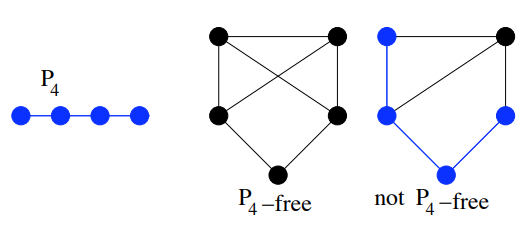
\includegraphics[keepaspectratio,alt={cograph\_p4.png}]{cograph_p4.png}}
\caption{cograph\_p4.png}
\end{figure}

A graph \(G\) is a cograph \(\iff\) \(G\) is \(P_4\)-free.

\subsection{Cotree}\label{cotree}

Let \(G\) be a cograph. The cotree \(T_G\) of \(G\) is the unique
decomposition tree that satisfies: 1. The root \(r\) of the tree
represents the graph \(G_r = G\) 2. Every leaf \(x\) of the tree
represents exactly one vertex of \(G\), and vice versa 3. Every internal
node \(x\) of the tree has at least two children, it is either labeled
\(+\) or \(\times\), and it represents an induced subgraph \(G_x\) of
\(G\), defined as follows: - if \(x\) is a \(+\)-node, then \(G_x\) is
the disjoint union of all graphs \(G_y\) where \(y\) is a child of \(x\)
- if \(x\) is a \(\times\)-node, then \(G_x\) is the join of all graphs
\(G_y\) where \(y\) is a child of \(x\) 4. Along the path from the root
\(r\) to any leaf, the labels of the internal nodes alternate between
\(+\) and \(\times\)

Any cograph \(G\) has a unique cotree. However, if we drop condition 4.,
there may be many trees representing \(G\).

An example is shown below.

\begin{figure}
\centering
\pandocbounded{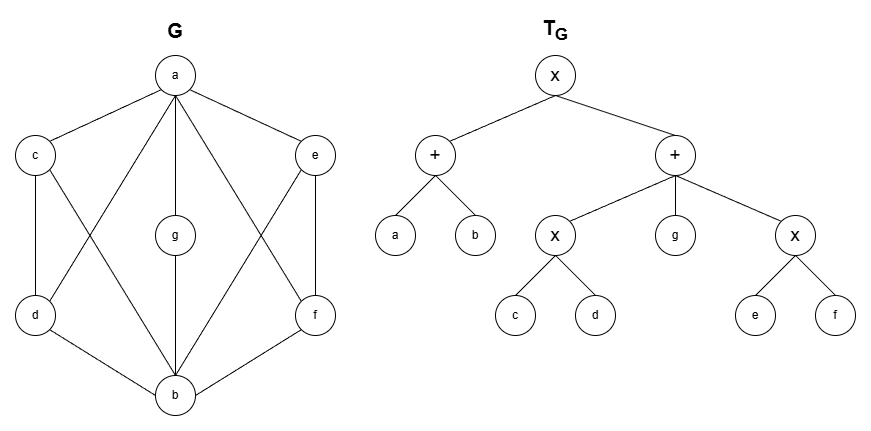
\includegraphics[keepaspectratio,alt={cotree\_example.png}]{cotree_example.png}}
\caption{cotree\_example.png}
\end{figure}

There is an algorithm for determining the cotree of a cograph, but it
will not be included here.

    \subsubsection{Colouring cographs}\label{colouring-cographs}

A colouring of a graph is an assignment of colors to the vertices of the
graph such that any two adjacent vertices are coloured differently.

A colouring using at most \(k\) colors is a \(k\)-colouring.

The chromatic number, \(\chi_G\) of a graph \(G\) is the smallest
integer \(k\) for which \(G\) has a \(k\)-colouring.

In general, this is complex, with no known polynomial-time algorithm.
However, for a cograph \(G\), its cotree \(T_G\) can be used to find its
chromatic number. A bottom-up approach is followed - only process node
\(x\) after first processing its children: - leaves: each leaf
represents a single vertex of \(G\). The chromatic number of a
single-vertex graph is 1. - union-nodes: if \(x\) is a \(+\)-node, then
\(\chi_{G_x}\) is the maximum of the chromatic numbers of the graphs
\(G_y\) , where \(y\) is a child of \(x\) - join-nodes: if \(x\) is a
\(\times\)-node, then \(\chi_{G_x}\) is the sum of the chromatic numbers
of the graphs \(G_y\) , where \(y\) is a child of \(x\).

This way, the last node processed is the root \(r\), which represents
the graph: \(G_r = G\).

As the number of nodes of T is \(O(n)\), and \(O(n)\) time is spent per
node, the total running time is polynomial.

    \section{The maximum-subarray
problem}\label{the-maximum-subarray-problem}

The maximum-subarray problem involves finding the maximum sum of a
contigous subarray of an array \(A\).

The brute force approach - checking all pairs of start and end indicies
- is \(\theta(n^2)\).

It is possible to do better, using divide-and-conquer. The idea is as
follows: - split the array in half at the midpoint \texttt{mid} - any
maximum subarray falls into one of three cases: - entirely in the left
half, \texttt{A{[}low...mid{]}} - entirely in the right half,
\texttt{A{[}mid...high{]}} - crossing the midpoint \texttt{mid} - the
first two cases can be solved recursively - to solve the third case: -
compute the max sum ending at \texttt{mid} from the left - compute the
max sum starting at \texttt{mid\ +\ 1} from the right - add the two sums
together

The running time of this is \(T(n) = \theta(n \log n)\).

    \section{The master theorem}\label{the-master-theorem}

The master theorem is used to solve reccurence relations, and is defined
as follows.

Let \(f(n)\) be a function on the natural numbers, and let \(T(n)\) be
defined by

\[
T(n) = aT\left(\frac{n}{b}\right) + f(n),
\]

for some constants \(a \ge 1\) and \(b > 1\). Then:

\begin{enumerate}
\def\labelenumi{\arabic{enumi}.}
\item
  If \(f(n) = O(n^{\log_b a - \epsilon})\) for some constant
  \(\epsilon > 0\), then \(T(n) = \Theta(n^{\log_b a})\).
\item
  If \(f(n) = \Theta(n^{\log_b a})\), then
  \(T(n) = \Theta(n^{\log_b a} \cdot \log n)\).
\item
  If \(f(n) = \Omega(n^{\log_b a + \epsilon})\) for some constant
  \(\epsilon > 0\), and if \(a \cdot f(n/b) \le c \cdot f(n)\) for some
  constant \(c < 1\) and for sufficiently large \(n\), then
  \(T(n) = \Theta(f(n))\).
\end{enumerate}

    \section{Matrix multiplication}\label{matrix-multiplication}

The problem we are interested in is multiplying two square matrices,
\(A, B \in \mathbb{R}^{n \times n}\) to get their product,
\(C \in \mathbb{R}^{n \times n}\).

Using the definition of matrix multiplication,
\(C_{ij} = \sum_{k=1}^n a_{ik} b_{kj}\), it can be performed in
\(\theta(n^3)\): - there are \(n^2\) elements - for each element, there
are \(n\) multiplications, and \(n-1\) additions;
\(n + (n-1) = \theta(n)\)

\subsection{Divide-and-conquer
approach}\label{divide-and-conquer-approach}

Suppose we have two \(n \times n\) matrices \(A\) and \(B\). For
simplicity, assume \(n\) is a power of 2 (so we can evenly split the
matrices).

Each matrix is partitioned into 4 equal-sized blocks, called block
matrices: \[
A = \begin{bmatrix} A_{11} & A_{12} \\ A_{21} & A_{22} \end{bmatrix}, \quad
B = \begin{bmatrix} B_{11} & B_{12} \\ B_{21} & B_{22} \end{bmatrix}, \quad
C = \begin{bmatrix} C_{11} & C_{12} \\ C_{21} & C_{22} \end{bmatrix}
\]

Here: - Each \(A_{ij}, B_{ij}, C_{ij}\) is a
\(\frac{n}{2} \times \frac{n}{2}\) matrix - For example, \(A_{11}\) is
the top-left quadrant of \(A\)

Then: \[
\begin{aligned}
C_{11} &= A_{11}B_{11} + A_{12}B_{21}, \\
C_{12} &= A_{11}B_{12} + A_{12}B_{22}, \\
C_{21} &= A_{21}B_{11} + A_{22}B_{21}, \\
C_{22} &= A_{21}B_{12} + A_{22}B_{22}
\end{aligned}
\]

Each of the smaller matrices can then be multiplied recursively.

The pseudocode for such an algorithm can be as follows:

\begin{verbatim}
MULT(A, B)

let C be a new n × n matrix
if n = 1 then
    c11 <- a11b11
else
    partition A, B, and C into the block matrices
    C11 <- MULT(A11, B11) + MULT(A12, B21)
    C12 <- MULT(A11, B12) + MULT(A12, B22)
    C21 <- MULT(A21, B11) + MULT(A22, B21)
    C22 <- MULT(A21, B12) + MULT(A22, B22)
return C
\end{verbatim}

    \subsubsection{Time complexity}\label{time-complexity}

The running time of this approach satisfies
\(T(n) = 8T(\frac{n}{2}) + \theta(n^2)\), since there are: - 8
multiplications of \(\frac{n}{2} \times \frac{n}{2}\) matrices, and - 4
matrix additions, each taking time
\(\theta(\frac{n}{2} \cdot \frac{n}{2}) = \theta(n^2)\)

Solving using the master theorem show that \(T(n) = \theta(n^3)\), so
this is not an improvement over using the definition.

    \subsection{Strassen's algorithm}\label{strassens-algorithm}

Strassen's algorithm builds on this divide-and-conquer approach: 1.
Divide \(A\), \(B\), and \(C\) into four parts as before - running time:
\(\theta(1)\) 2. Create 10 auxiliary matrices
\(S_1, \ldots , S_{10} \in \mathbb{R}^{n/2 \times n/2}\), obtained by
sums or differences of \(A_{11}, \ldots , B_{22}\). - running time:
\(\theta(n^2)\) 3. Using all the matrices available, recursively compute
seven product matrices
\(P_1, \ldots , P7 \in \mathbb{R}^{n/2 \times n/2}\) - running time:
\(7T(n/2)\) 4. Compute \(C_{11}, \ldots , C_{22}\) by adding/subtracting
combinations of \(P_1, \ldots , P7\). - running time: \(\theta(n^2)\)

The running time of this approach satisfies
\(T(n) = 7T(\frac{n}{2}) + \theta(n^2)\)

Using the master theorem, we obtain:
\[T(n) = \theta(n^{\log_2 7}) = \theta(n^{2.8074})\]

    \section{Rod cutting problem}\label{rod-cutting-problem}

The rod cutting problem is as follows.

Given: - A rod of length \(n\). - A price list \(p_i\) for
\(i = 1, \ldots\ n\) where \(p_i\) is the selling price of a rod of
length \(i\).

Determine the maximum revenue \(r_n\) obtained by cutting up the rod and
selling the pieces.

\subsection{Brute force}\label{brute-force}

One way to solve this problem is by brute force - trying all possible
integer combinations (we assume the rod must be cut into integer-length
parts).

An integer partition of a positive integer \(n\) is a list of positive
integers \(a_1, \ldots , a_k\) such that
\(a_1 \leq a_2 \leq \ldots \leq a_k\) and \(\sum_{i=1}^k a_i = n\).

The number of integer partitions of \(n\) increases exponentially with
\(n\).

Therefore, the brute force method has an exponential running time, and
is impractical.

    \subsection{Optimal substructure}\label{optimal-substructure}

As a general solution,
\[r_n = \text{max} \{p_i + r_{n-i}: 1 \leq i \leq n\}\]

Essentially, the maximum revenue from a rod of length \(n\) is obtained
by choosing the best first cut length \(i\), earning \(p_i\) from that
piece, and then optimally cutting the remaining rod of length \(n-i\).

Therefore, to solve the original problem of size \(n\), we solve
independent smaller problems of the same type, but of smaller sizes.

Optimal substructure means that an optimal solution to a problem can be
constructed from optimal solutions to its subproblems (which may be
solved independently).

    \subsection{Recursive top-down
implementation}\label{recursive-top-down-implementation}

An algorithm that relies on optimal substructure is given in pseudocode
below:

\begin{verbatim}
ROD(p, n)

if n == 0 then
    return 0
q <- -1
for i <- 1 to n do
    q <- max{q, p[i] + ROD(p, n - i)}
return q
\end{verbatim}

This algorithm: - tries every possible first cut - solves the remaining
subproblem recursively - then chooses the best option

However, this algorithm recomputes the same values many times, and
therefore the time complexity is exponential.

    \subsection{Dynamic programming}\label{dynamic-programming}

Rather than re-solving the same subproblem repeatedly, the subproblems
can be arranged so that each subproblem is solved only once, with its
solution stored. If the solution is needed thereafter, it is retrieved
instead of recomputed.

Dynamic programming implements this idea by using additional memory to
save computation time. It is therefore an example of time-memory trade
off.

A dynamic programming algorithm runs in polynomial time when both: - the
number of distinct subproblems involved is polynomial - each subproblem
can be solved in polynomial time

Note that for any algorithm that uses subproblems, the subproblems have
to be independent. Two subproblems are independent if the solution to
one subproblem does not affect the solution to another subproblem of the
same problem.

Dynamic programming is effective because it utilises both: - optimal
substructure (where the solution to a problem can be constructed from
optimal solutions to its subproblems), and - overlapping subproblems
(where the same subproblem appears in multiple larger problems)

It uses memoization, which is the process of caching the results of
function calls (subproblem solutions) so that repeated calls with the
same arguments can return the cached result instead of recomputing it.

    \subsubsection{Top-down implementation with
memoization}\label{top-down-implementation-with-memoization}

The top-down implementation from earlier can be improved using
memoization.

The procedure is still written recursively in a natural manner, but
modified to save the result of each subproblem (in an array).

Them, when the procedure needs to solve a subproblem, it checks if it
has previously solved this subproblem; if not, the procedure computes
the value in the usual manner.

We say the recursive procedure has been memoized: it remembers what
results it has computed previously.

The pseudocode for this is given below.

\begin{verbatim}
MEMOIZED-ROD(p, n)
Let r[0..n] be a new array
for i <- 0 to n do
    r[i] <- -1
return MEMOIZED-ROD-AUX(p, n, r)

MEMOIZED-ROD-AUX(p, n, r)
if r[n] >= 0 then
    return r[n]   // r[n] has been previously computed
if n == 0 then
    q <- 0   // the returned value r[0]
else
    q <- -1
    for i <- 1 to n do   // compute r[n]
        q <- max{q, p[i] + MEMOIZED-ROD-AUX(p, n - i, r)}
r[n] <- q
return q
\end{verbatim}

    \subsubsection{Bottom-up implementation}\label{bottom-up-implementation}

Another approach to implement dynamic programming is the bottom-up
method.

It depends on the idea of the `size' of a subproblem, such that solving
any particular subproblem relies on solving smaller subproblems.

The subproblems are sorted by size and solved in size order, smallest
first, with the solutions saved.

Each subproblem is solved only once, and when it is first seen, all of
its prerequisite subproblems have already been solved.

The pseudocode for this is given below:

\begin{verbatim}
BOTTOM-UP-ROD(p, n)
Let r[0..n] be a new array
r[0] <- 0
for j <- 1 to n do
    q <- -1
    for i <- 1 to j do
        q <- max{q, p[i] + r[j - i]}   // r[j - i] is known
    r[j] <- q
return r[n]
\end{verbatim}

    \paragraph{Running time}\label{running-time}

For rod cutting, both the top-down and bottom-up dynamic programming
approaches have a worst case running time of \(\theta(n^2)\).

This is easy to see for the bottom-up approach, since it contains a
(single) nested for loop.

The top-down approach solves each subproblem for sizes
\(0, 1, \ldots, n\) once. Therefore, to solve a problem of size \(n\): -
the for loop iterates \(n\) times - the total number of iterations is
the sum \$ 1 + 2 + \ldots + n\$, an arithmetic series, giving
\(\theta(n^2)\)

For other problems, both approaches typically have the same complexity,
but: - the bottom-up approach has lower constants, due to less overhead
for procedure calls - top-down may sometimes avoid solving certain
subproblems entirely, if they are never needed in the recursion tree.
This can make it faster in practice for some sparse problems

    \section{Matrix chain multiplication}\label{matrix-chain-multiplication}

Let \(A\) be a \(p \times q\) matrix, and \(B\) be a \(q' \times r\)
matrix, i.e., \[
A =
\\begin{pmatrix}
a_{1,1} & a_{1,2} & \\dots & a_{1,q} \\
a_{2,1} & a_{2,2} & \\dots & a_{2,q} \\
\\vdots & \\vdots & \\ddots & \\vdots \\
a_{p,1} & a_{p,2} & \\dots & a_{p,q}
\\end{pmatrix}, \\quad
B =
\\begin{pmatrix}
b_{1,1} & b_{1,2} & \\dots & b_{1,r} \\
b_{2,1} & b_{2,2} & \\dots & b_{2,r} \\
\\vdots & \\vdots & \\ddots & \\vdots \\
b_{q,1} & b_{q,2} & \\dots & b_{q,r}
\\end{pmatrix}
\] The product \(C = AB\): - is not defined if \(q \\neq q'\) - is the
\(p \\times r\) matrix if \(q = q'\), where
\[c_{i,j} = \\sum_{k=1}^{q} a_{i,k} b_{k,j}\]

This matrix has \(p \\cdot r\) entries, and for each entry, there are
\(q\) multiplication and \(q-1\) additions = \(\\theta(q)\) operations
per entry. - the runtime of this matrix multiplication is
\(\\theta(pqr)\)

Matrix multiplication is associative: - the multiplication ordering does
not change the product - e.g,
\(A_1 A_2 A_3 = (A_1(A_2 A_3)) = ((A_1 A_2)A_3)\)

Even though the result is the same, one order of multiplication may
involve significantly fewer multiplications than another.

For example, take three matricies:
\[ A_1: 10 \\times 100, \\quad A_2: 100 \\times 5, \\quad A_3: 5 \\times 50\]

There are two ways of parenthesizing: - \((A_1 A_2)A_3\) requires -
\((10 \\times 100 \\times 5) + (10 \\times 5 \\times 50) = 7,500\)
multiplications - \(A_1(A_2 A_3)\) requires -
\((100 \\times 5 \\times 50) + (10 \\times 100 \\times 50) = 75,000\)
multiplications

The matrix chain multiplication problem is defined as follows.

Given a sequence (chain) \(⟨A_1, \\ldots , A_n⟩\) of \(n\) matrices,
where \(A_i\) has dimensions \(p_{i-1} \\times p_i\), determine the
optimal parenthesization of the product \(A_1 A_2 \\ldots A_n\) that
minimises the total number of scalar multiplications.

A product of matrices \[ A_1 A_2 \\ldots A_N\] is fully parenthesized if
it is: - either a single matrix, - or the product of two fully
parenthesized matrix products, surrounded by parentheses

Let \(P(n)\) denote the number of ways to parenthesize a product of
\(n\) matrices.

If the product is fully parenthesized, then: - it is the product of two
fully parenthesized sub-products - the split of these two sub-products
occurs between the \(k\)th and \((k + 1)\)st matrices, where
\(1 \\leq k \\leq n - 1\)

This provides the recurrence: \[ 
P(n) =
\\begin{cases}
1, & \\text{if } n = 1 \\\\[2mm]
\\sum_{k=1}^{n-1} P(k) \\, P(n-k), & \\text{if } n \\ge 2
\\end{cases}
\]

    \subsection{Applying dynamic
programming}\label{applying-dynamic-programming}

To use dynamic programming, follow a four-step sequence: 1. Characterise
the structure of an optimal solution. 2. Recursively define the value of
an optimal solution. 3. Compute the value of an optimal solution. 4.
Construct an optimal solution from computed information.

    \subsubsection{Structure of an optimal
solution}\label{structure-of-an-optimal-solution}

To optimally parenthesize \(A_i \ldots A_j\), suppose that we split the
product between \(A_k\) and \(A_{k+1}\): - both parenthesizations of
\(A_i \ldots A_k\) and \(A_{k+1} \ldots A_j\) must be optimal

The cost of the optimal solution for \(A_i \ldots A_j\) is the sum of: -
the cost to optimally parenthesize \(A_i \ldots A_k\) - the cost to
optimally parenthesize \(A_{k+1} \ldots A_j\) - the cost of multiplying
them together

    \subsubsection{Recursive definition of the value of an optimal
solution}\label{recursive-definition-of-the-value-of-an-optimal-solution}

Let \(m[i, j]\) be the minimum number of multiplications required to
compute \(A_i \ldots A_j\).

The goal is to compute \(m[1, n]\).

\(m[1, n]\) can be computed recursively, for \(i \leq j\): \[
m[i,j] =
\begin{cases}
0, & \text{if } i = j, \\[2mm]
\displaystyle \min_{i \le k < j}
\left\{ m[i,k] + m[k+1,j] + p_{i-1} p_k p_j \right\},
& \text{if } i < j .
\end{cases}
\]

There are two cases: - the base case: if \(i = j\), then \(m[i,j] = 0\),
since a single matrix needs no multiplication - the recursive case: if
\(i < j\), then: - check all possible places to split - use the minimum
of all of these

    \subsubsection{Computing optimal costs}\label{computing-optimal-costs}

There are only a few distinct subproblems: - one for every pair of \(i\)
and \(j\), so there are \(\theta(n^2)\) subproblems - there are many
overlapping subproblems

A bottom-up approach can be used: - computing \(m[i, j]\) for a product
of \(j - i + 1\) matrices only uses values for products of fewer than
\(j - i + 1\) matrices. - order matrices by their chain length
\(\ell = j - i + 1\) - this is just the number of matricies being
multiplied in the subproblem - store the answers in a table
\(m[1 \ldots n, 1 \ldots n]\) - starting from the shortest chain length
(the smallest number of matricies in the product), calculcate \(m[i,j]\)
- first fill \(m[i,i]\) = 0 - then compute chains of length 2, then
length 3 etc. until length \(n\) - for each chain, try every possible
split and choose the cheapest

Pseudocode for this is given below:

\begin{verbatim}
MATRIX-CHAIN-ORDER(p)
Let m[1..n, 1..n] be a new table
for i <- 1 to n do
    m[i, i] <- 0
for L <- 2 to n do
    for i <- 1 to n - L + 1 do
        j <- i + L - 1
        m[i, j] <- \infty
        for k <- i to j - 1 do
            m[i, j] <- min{m[i, j], m[i, k] + m[k + 1, j] + p_{i-1} p_k p_j}
return m
\end{verbatim}

So far, we have determined the minimum number of multiplications, but
not where the parenthesis should be placed to achieve it.

However, it is easy to modify the solution to keep track of where to
place the parenthesis: - for every \(i\) and \(j\), it is enough to
remember the cut point \(k\), where we cut the product
\(A_i \ldots A_j\) into \(A_i \ldots A_k\) and \(A_{k+1} \ldots A_j\) -
an additional array \(s[i, j]\) can be used to keep track of all those
\(k\)'s

\begin{verbatim}
MATRIX-CHAIN-ORDER(p)
Let m[1..n, 1..n] and s[1..n - 1, 2..n] be new tables
for i <- 1 to n do
    m[i, i] <- 0
for L <- 2 to n do
    for i <- 1 to n - L + 1 do
        j <- i + L - 1
        m[i, j] <- \infty
        for k <- i to j - 1 do
            q <- min{m[i, j], m[i, k] + m[k + 1, j] + p_{i-1} p_k p_j}
            if q < m[i, j] then
                m[i, j] <- q
                s[i, j] <- k
return m
\end{verbatim}

    \subsubsection{Constructing an optimal
solution}\label{constructing-an-optimal-solution}

The table \(s[1..n - 1, 2..n]\) hold the information to print out the
right parenthesization.

\begin{verbatim}
Algorithm PRINT-PAR(s, i, j)
if i == j then
    print "Ai"
else
    print "("
    PRINT-PAR(s, i, s[i, j])
    PRINT-PAR(s, s[i, j] + 1, j)
    print ")"
\end{verbatim}

This part has running time \(O(n)\).

    \paragraph{Running time}\label{running-time}

The main algorithm contains three nested for loops, therefore the
running time of the algorithm is \(O(n^3)\).

It can further be shown that the running time is actually
\(\theta(n^3)\).

    \section{Longest common subsequence}\label{longest-common-subsequence}

The longest common subsequence problem is as follows.

Given two sequences, find the longest sequence of characters (longest
common subsequence) that: - appears in both sequences - appears in the
same order - is not necessarily contiguous (i.e., characters don't have
to be next to each other)

For example, for the strings \texttt{S1} and \texttt{S2} below,
\texttt{S3} is the longest common subsequence:

\begin{figure}
\centering
\pandocbounded{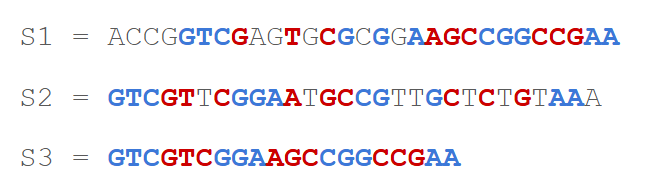
\includegraphics[keepaspectratio,alt={LCS example}]{lcs_example.png}}
\caption{LCS example}
\end{figure}

Formally, given a sequence \(X = \langle x_1, \dots, x_m \rangle\),
another sequence \(Z = \langle z_1, \dots, z_k \rangle\) is a
subsequence of \(X\) if there exist indices \(i_1 < i_2 < \dots < i_k\)
such that\\
\(z_1 = x_{i_1}, \; z_2 = x_{i_2}, \; \dots, \; z_k = x_{i_k}\). - the
elements do not have to be consecutive --- only the order must be
preserved

A common subsequence of \(X\) and \(Y\) is a subsequence of both \(X\)
and \(Y\).

    \subsection{Brute-force}\label{brute-force}

A possible brute-force approach is to: - enumerate all subsequences
\(Z\) of \(X\) - check whether \(Z\) is also a subsequence of \(Y\) -
keep track of the longest subsequence that appears in both

If \(X\) has \(m\) indicies, there are \(2^m\) subsets - therefore, the
brute force approach has exponential running time

    \subsection{Dynamic programming}\label{dynamic-programming}

Let \(X = \langle x_1, x_2, \dots, x_n \rangle\), and let the \(i\)th
prefix of \(X\) be \(X_i = \langle x_1, x_2, \dots, x_i \rangle\).

    \subsubsection{Optimal substructure}\label{optimal-substructure}

Let \(Z = \langle z_1, \dots, z_k \rangle\) be an LCS of
\(X = \langle x_1, \dots, x_m \rangle\) and
\(Y = \langle y_1, \dots, y_n \rangle\).

\begin{enumerate}
\def\labelenumi{\arabic{enumi}.}
\tightlist
\item
  If \(x_m = y_n\), then:

  \begin{itemize}
  \tightlist
  \item
    \(z_k = x_m = y_n\)
  \item
    \(Z_{k-1}\) is an LCS of \(X_{m-1}\) and \(Y_{n-1}\)
  \end{itemize}
\item
  If \(x_m \ne y_n\), then:

  \begin{itemize}
  \tightlist
  \item
    \(z_k \ne x_m\) implies that \(Z\) is an LCS of \(X_{m-1}\) and
    \(Y\)
  \end{itemize}
\item
  If \(x_m \ne y_n\), then:

  \begin{itemize}
  \tightlist
  \item
    \(z_k \ne y_n\) implies that \(Z\) is an LCS of \(X\) and
    \(Y_{n-1}\)
  \end{itemize}
\end{enumerate}

In words, this means: - look at the last character of \(X\) and \(Y\) -
if the last characters match: - this character must be the last
character in the LCS, because if it weren't used, we could append it and
get a longer common subsequence (contradiction) - everything before it,
\(Z_{k-1}\), must be an LCS of the prefixes \(X_{m-1}\) and \(Y_{n-1}\)
- if the last characters don't match: - at least one of them is not part
of the LCS - if the LCS does not end with the last character of \(X\),
then discarding this character \(X_m\) does not affect the LCS -
therefore, \(Z\) is an LCS of \(X_{m-1}\) and \(Y\) - if the LCS does
not end with the last character of \(Y\), then discarding this character
\(Y_n\) does not affect the LCS - therefore, \(Z\) is an LCS of \(X\)
and \(Y_{n-1}\)

Therefore, there is an optimal substructure: - an LCS of \(X\) and \(Y\)
contains within it an LCS of some prefixes of \(X\) and \(Y\)

One or two subproblems have to be examined each time: 1. if
\(x_m = y_n\) we must find an LCS of \(X_{m-1}\) and \(Y_{n-1}\) 2. if
\(x_m \neq y_n\) we have to find: - an LCS of \(X_{m-1}\) and \(Y\) - an
LCS of \(X\) and \(Y_{n-1}\)\\
- keep whichever is longer

There is also the overlapping subproblems property: - we may need to
find LCS's of \(\{X_{m-1}, Y\}\) and of \(\{X, Y_{n-1}\}\) - each of
these subproblems has the subproblem of finding an LCS of
\(\{X_{m-1}, Y_{n-1}\}\) - therefore, many other subproblems share
common subproblems

    \subsubsection{Recursive solution}\label{recursive-solution}

Let \(c[i, j]\) be the length of an LCS of the prefixes \(X_i\) and
\(Y_j\).

Therefore, \[
c[i, j] =
\begin{cases}
0 & \text{if } i = 0 \text{ or } j = 0, \\
c[i - 1, j - 1] + 1 & \text{if } i, j > 0 \text{ and } x_i = y_j, \\
\max\{c[i, j - 1], \, c[i - 1, j]\} & \text{if } i, j > 0 \text{ and } x_i \ne y_j.
\end{cases}
\]

Unlike the rod cutting and the matrix chain multiplication problems,
here we rule out some subproblems based on the conditions of the problem
(i.e.~\(x_i = y_j\) or \(x_i \neq y_j\)).

Used directly, this recursive equation gives an exponential time
recursive algorithm. However: - every recursive call is of the form
\(\text{c}[i,j]\) - so a subproblem is identified by the pair \((i,j)\),
where \(i \in \{0, 1, \ldots, m\}\) and \(j \in \{0, 1, \ldots, n\}\) -
so the number of distinct subproblems = \((m+1)(n+1) = \theta(mn)\)

Therefore, using dynamic programming to only solve each subproblem once
and store the result for reuse if needed, reduces the algorithm to
polynomial time, more specifically, \(\theta(mn)\).

    \subsubsection{Computing the length of an
LCS}\label{computing-the-length-of-an-lcs}

A bottom-up approach can be used: - create a length table
\(c[0 \ldots m, 0 \ldots n]\) - \(c[i,j]\) is length of the LCS of
prefixes \(X_i\) and \(Y_j\) - create a direction table
\(b[1 \ldots m, 1 \ldots n]\) - \(b[i,j]\) is a pointer that tells us
how the optimal value in \(c[i, j]\) was obtained - this table is used
later to reconstruct the actual LCS - initialise the base cases: - for
all \(i\), set \(c[i, 0] = 0\) - for all \(j\), set \(c[0, j] = 0\) -
fill the tables in row by row - once the table is complete, the length
of the LCS is stored in: \(c[m,n]\)

Pseudocode for this is given below:

\begin{verbatim}
LCS(X, Y)
Let b[1..m, 1..n] and c[0..m, 0..n] be new tables
for i <- 0 to m do c[i, 0] <- 0
for j <- 0 to n do c[0, j] <- 0
for i <- 1 to m do
    for j <- 1 to n do
        if xi == yj then
            c[i, j] <- c[i-1, j-1] + 1
            b[i, j] <- "diag"  // upper-left subproblem
        else if c[i-1, j] >= c[i, j-1] then
            c[i, j] <- c[i-1, j]
            b[i, j] <- "up"  // upper subproblem
        else
            c[i, j] <- c[i, j-1]
            b[i, j] <- "left"  // left subproblem
return c and b
\end{verbatim}

\subsubsection{Constructing an LCS}\label{constructing-an-lcs}

To recover the actual subsequence (not just its length): - start at cell
\((m, n)\) - follow the pointers in \(b\): - whenever we see a diagonal
pointer (\texttt{diag}): - output the corresponding character - move to
\((i-1, j-1)\) - if the pointer is up (\texttt{up}), move to
\((i-1, j)\) - if the pointer is left (\texttt{left}), move to
\((i, j-1)\) - stop when you reach the top row or leftmost column - the
characters collected (in reverse order) form the LCS

\begin{verbatim}
PRINT-LCS(b, X, i, j)
if i == 0 or j == 0 then
    return ""
if b[i, j] == "diag" then
    PRINT-LCS(b, X, i-1, j-1)
    print xi
else if b[i, j] == "up" then
    PRINT-LCS(b, X, i-1, j)
else
    PRINT-LCS(b, X, i, j-1)
\end{verbatim}

    \section{Matching in graphs}\label{matching-in-graphs}

Let \(G = (V, E)\) be an undirected graph.

When modeling a real-world application, usually: - vertices \(v \in V\)
represent some objects of interest, e.g.~cities on a map - edges
\(e \in E\) represent relations between pairs of vertices, e.g.~roads
between cities

However, often the edges become the interesting objects to study - an
edge unites or matches two vertices

A matching \(M \subseteq E\) in \(G\) is an independent
(non-conflicting) set of edges, i.e.~a set of edges where no two edges
share a common vertex. No object is used twice; there are no conflicts,
as each object is matched with at most one partner.

Matchings are useful as many real-world problems are about making
non-conflicting pairings. - for example, suppose there is a graph where
each vertex represents a football team, and each edge represents a
potential game between two teams - if a number of football games are to
be scheduled at the same time, a matching would be required, as a team
can only play one other team at a time

A bipartite graph is a graph where the verticies can be split into two
disjount groups, such that all edges go between the two groups, and
never within the same group. Such a graph can be two-coloured.

Formally, a graph \(G=(V,E)\) is bipartite if its vertex set \(V\) can
be partitioned into two sets, \(V = X \cup Y\) such that -
\(X \cap Y = \emptyset\) (they don't overlap) - every edge connects a
vertex in \(X\) to a vertex in \(Y\) - no edge connects two vertices
both in \(X\) - no edge connects two vertices both in \(Y\)

Many assignment problems can be formulated as finding a special matching
in a bipartite graph \(G = (X \cup Y, E)\). - for example, verticies in
\(X\) are workers, and verticies in \(Y\) are projects to be assigned to
workers; each edge represents a job a worker is able to do

A matching \(M\) is called: - maximal, if \(M\) is not a proper subset
of any other matching \(M'\) in \(G\) - maximum, if no other matching
\(M'\) in \(G\) contains a strictly greater number of edges - perfect,
if every vertex of \(G\) is an endpoint of an edge in \(M\)

The matching number \(\nu_G\) of \(G\) is the size of a maximum matching
in \(G\).

Note: - Every maximum matching is also maximal - A maximal matching is
not necessarily maximum - A perfect matching is always maximum

\begin{figure}
\centering
\pandocbounded{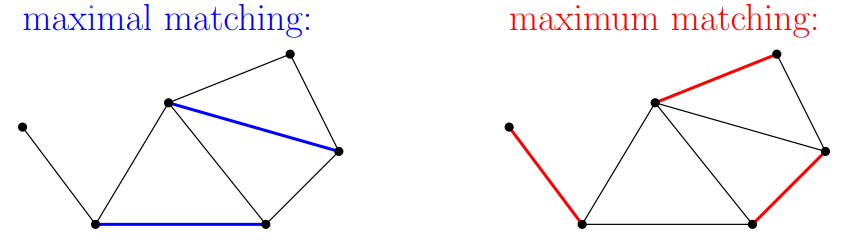
\includegraphics[keepaspectratio,alt={matching example}]{matching_example.png}}
\caption{matching example}
\end{figure}

    \subsection{Alternating paths and
cycles}\label{alternating-paths-and-cycles}

Let \(G = (V, E)\) be a graph and \(M\) be a matching in \(G\).

Let \(P = (v_0, v_1, \ldots , v_k)\) be a simple path with edges
\(e_1 = v_0 v_1, e_2 = v_1 v_2, \ldots , e_k = v_{k-1} v_k\).\\
Then: - P is an \(M\)-alternating path if the edges
\(e_1, e_2, \ldots , e_k\) are alternately in \(M\) and in
\(E \setminus M\).
\pandocbounded{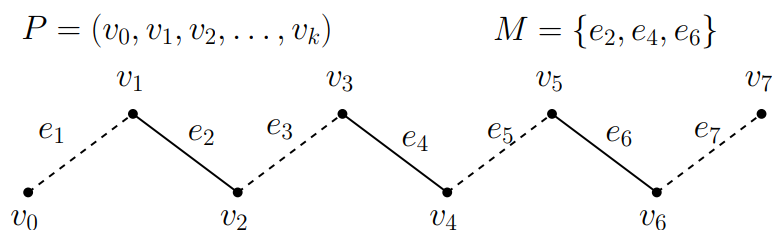
\includegraphics[keepaspectratio,alt={m alternating}]{m_alternating.png}}
- P is an \(M\)-augmenting path if \(P\) is \(M\)-alternating and
neither \(v_0\) nor \(v_k\) is covered by \(M\) - this requires
\(M = \{e_2, e_4, \ldots , e_{k-1}\}\) - therefore, \(k\) is odd in an
augmenting path

Similarly, a cycle \(C\) in \(G\) is an \(M\)-alternating cycle if its
edges alternately belong to \(M\) and \(E \setminus M\).

A vertex \(u\) is matched by \(M\) if it is the end-vertex of an edge in
\(M\); otherwise \(u\) is unmatched by \(M\).

For two sets \(A\) and \(B\), the symmetric difference is the set
\(A \otimes B = (A \setminus B) \cup (B \setminus A)\). - for example:\\
Let \(A = \{1,2,3,4\}\) and \(B = \{3,4,5,6\}\)\\
Then:\\
\(A \setminus B = \{1,2\}\)\\
\(B \setminus A = \{5,6\}\)\\
so \(A \otimes B = \{1,2,5,6\}\)

    \subsubsection{Running time}\label{running-time}

Since we only explore each edge once, the algorithm for finding an
augmenting path runs in \(O(|E|)\) time.

Each occasion results in a matching that has one more edge than the
previous matching. The largest possible matching has \(\frac{|V|}{2}\)
verticies, so the augmenting path algorithm is run at most
\(\frac{|V|}{2}\) times.

Therefore, the total running time of the algorithm for finding a maximum
matching in a bipartite graph is \(O(|E||V|)\) time.

    \section{Dijkstra's Algorithm}\label{dijkstras-algorithm}

\subsection{Adjacency matrix}\label{adjacency-matrix}

An adjacency matrix can be used to represent a graph with edge weights:
- a square matrix is used - rows and columns are labelled with the
vertices

The entry in row \(i\) and column \(j\) is: - \(w\) if there is an edge
of weight \(w\) from \(i\) to \(j\), - \(0\) if there is no edge.

    \subsection{Shortest path}\label{shortest-path}

The weight (or length) of a path from a vertex \(u\) to a vertex \(v\)
is the sum of the weights of the edges in the path.\\
Note that a weight may be negative.

The shortest path (i.e.~with least weight) between \(u\) and \(v\) is
denoted \(\delta (u, v)\). If there is no path, then
\(\delta (u, v) = \infty\).

    \subsection{Single-source shortest paths
problem}\label{single-source-shortest-paths-problem}

The single-source shortest paths problem involves finding the shortest
path from a specific source vertex \(s\) to all other verticies in the
graph.

    \subsection{Relaxing an edge}\label{relaxing-an-edge}

Relaxing an edge means checking whether going through that edge gives a
shorter path to a vertex, and updating the distance if it does.

    \subsection{Dijkstra's algorithm}\label{dijkstras-algorithm}

\begin{enumerate}
\def\labelenumi{\arabic{enumi}.}
\tightlist
\item
  Initialisation

  \begin{itemize}
  \tightlist
  \item
    the node \(A\) is the source node
  \item
    the set \(S\) stores the vertices \(v\) for which \(\delta(A, v)\)
    has been found (initially empty)
  \item
    the set \(Q\) stores all the other vertices (initially contains all
    vertices)
  \item
    \(d(v)\) is an estimate of \(\delta(A, v)\)
  \item
    \(d(A) = 0\) (initially infinite for all other vertices)
  \end{itemize}
\item
  While \(Q\) is not empty:

  \begin{itemize}
  \tightlist
  \item
    remove from \(Q\) the vertex \(u\) for which \(d(u)\) is minimum
  \item
    add this vertex \(u\) to \(S\)
  \item
    relax all edges leaving \(u\)
  \end{itemize}
\end{enumerate}

The running time of Dijkstra's algorithm is \(O(V^2)\).

    \subsection{Properties of shortest paths and
relaxation}\label{properties-of-shortest-paths-and-relaxation}

\begin{itemize}
\tightlist
\item
  Triangle Inequality

  \begin{itemize}
  \tightlist
  \item
    For all edges \((u, v)\), we have
    \(\delta(s, v) \leq \delta(s, u) + w(u, v)\).
  \end{itemize}
\item
  Optimal Substructure

  \begin{itemize}
  \tightlist
  \item
    Any subpath of a shortest path is also a shortest path.
  \end{itemize}
\item
  Upper Bound Property

  \begin{itemize}
  \tightlist
  \item
    For every vertex \(v\), we always have \(d(v) \geq \delta(s, v)\).
  \end{itemize}
\item
  No-path Property

  \begin{itemize}
  \tightlist
  \item
    If \(\delta(s, v) = \infty\), then we have \(d(v) = \infty\) at
    every iteration.
  \end{itemize}
\item
  Convergence Property

  \begin{itemize}
  \tightlist
  \item
    If there is a shortest path from \(s\) to \(v\) including the edge
    \((u, v)\) and if \(d(u) = \delta(s, u)\), then we obtain
    \(d(v) = \delta(s, v)\) when \((u, v)\) is relaxed.
  \end{itemize}
\end{itemize}

    \section{Flow networks}\label{flow-networks}

Take a scenario where: - material is transfered in a network from a
``source'' to a ``sink'' - source produces material at a steady rate,
sink consumes at same rate

For example, water through a system of pipes or current through an
eletrical network.

Edges have a given capacity - the maximum material transfer per unit of
time

Vertices (other than source/sink) are ``junctions'': - material flows
through them without collecting in them - entering rate = exiting rate
(flow conservation)

    \subsection{Maximum-flow problem}\label{maximum-flow-problem}

The maximum-flow problem involves computing the greatest possible rate
of transportation from source to sink in a flow network.

A flow network is defined by a directed graph \(G = (V,E)\), with: - two
distinguished vertices: source \(s\) and sink \(t\) - each edge
\((u, v) \in E\) has non-negative capacity \(c(u, v) \geq 0\) - if
\((u, v) \not\in E\), we assume \(c(u, v) = 0\).

We assume that every vertex lies on some path from \(s\) to \(t\): - for
each \(v \in V\), there is a path \(s \leadsto v \leadsto t\) -
therefore, \(G\) is connected, so \(|E| \geq |V| - 1\)

    \subsubsection{Flow}\label{flow}

A flow in \(G\) is a real-valued function
\(f : V \times V \rightarrow \mathbb{R}\) that satisfies three
properties: - Capacity constraint: - For all \(u, v \in V\), we require
\(f(u, v) \leq c(u, v)\) - Flow from one vertex to another must not
exceed given capacity. - Skew symmetry: - For all \(u, v \in V\), we
require \(f(u, v) = -f(v, u)\) - Flow from vertex \(u\) to vertex \(v\)
is negative of flow in reverse direction. - Flow conservation: For all
\(u \in V - {s,t}\), we require - \(\sum_{v \in V} f(u, v) = 0\) - Total
flow out of a vertex (other than source or sink) is 0.

\(f(u, v)\) is called the flow from \(u\) to \(v\). It can be positive,
zero, or negative.

\paragraph{Total flow}\label{total-flow}

The total positive flow entering vertex \(v\) is
\[\sum_{u \in V: f(u, v)>0} f(u, v)\]

The total positive flow leaving vertex \(u\) is
\[\sum_{v \in V: f(u, v)>0} f(u, v)\]

The total net flow at a vertex \(v\) is: - total positive flow leaving
\(v\) - total positive flow entering \(v\)

Total net flow is: - positive at source - negative at sink - 0 at all
other verticies

\paragraph{Flow value}\label{flow-value}

The value of flow \(f\) is defined as the total flow leaving the source
(and thus entering the sink): \[|f| = \sum_{v\in V} f(s,v)\]

    \subsubsection{Implicit summation}\label{implicit-summation}

Let \(X, Y \subseteq V\). Then:
\[f(X,Y) = \sum_{x \in X} \sum_{y \in Y} f(x,y)\]

Commonly occuring identities: - For all \(X \subseteq V\), we have
\(f(X, X) = 0\) - Because each \(f(u, v)\) and \(f(v, u) = -f(u, v)\)
cancel each other. - For all \(X, Y \subseteq V\), we have
\(f(X, Y) = -f(Y, X)\) - Generalization of f (X, X) = 0, same reasoning.
- For all \(X, Y , Z \subseteq V\) with \(X \cap Y = \emptyset\), we
have - \(f(X \cup Y, Z) = f(X, Z) + f(Y , Z)\) -
\(f(Z, X \cup Y) = f(Z, X) + f(Z, Y)\) - Split summation into two: one
over \(X\), one over \(Y\)

    \subsection{The Ford-Fulkerson method}\label{the-ford-fulkerson-method}

The Ford-Fulkerson method is an iterative method for solving the maximum
flow problem: 1. Start with \(f(u, v) = 0\) for all \(u, v \in V\) 2. At
each iteration, increase flow value by finding an augmenting path --- a
path from source to sink along which we can increase flow --- and then
augment flow along this path. 3. Repeat until no augmenting path can be
found

    \subsubsection{Residual networks}\label{residual-networks}

The residual network consists of edges that can admit more flow.

Consider vertices \(u\) and \(v\). The amount of additional flow we can
push from \(u\) to \(v\) before exceeding capacity \(c(u, v)\) is the
residual capacity of \((u, v)\): - \(c_f(u, v) = c(u, v) - f(u, v)\)

Note: When flow \(f(u, v)\) is negative, then residual capacity
\(c_f(u, v)\) is greater than \(c(u, v)\).

Given flow network \(G = (V, E)\) and flow \(f\), the residual network
of \(G\) induced by \(f\) is \(G_f = (V, E_f)\) with
\[E_f = {(u, v) \in V \times V : c_f (u, v) > 0}\] i.e.~each residual
edge that can admit flow that is strictly positive.

Let \(G = (V, E)\) be a flow network, \(f\) be a flow in \(G\), \(G_f\)
be the residual network of \(G\) induced by \(f\), and let \(f'\) be a
flow in \(G_f\). Then the flow sum \(f + f'\) with

    \subsubsection{Augmenting path}\label{augmenting-path}

An augmenting path is a path in the residual graph from the source \(s\)
to the sink \(t\) where every edge has residual capacity \(> 0\).

Along this path, you can increase the flow by the minimum residual
capacity on the path.

    \subsubsection{Cuts}\label{cuts}

A cut \((S,T)\) is a partition of all the nodes \(V\) into two sets: -
\(S\) --- contains the source \(s\) - \(T\) --- contains the sink \(t\)

Every node is in exactly one of the two sets: \(S \cup T = V\),
\(S \cap T = \emptyset\)

If \(f\) is a flow in \(G\), then \(f(S,T)\) is the net flow across cut
\((S,T)\); its capacity is \(c(S,T)\). - net flow includes negative
flows across the cut; capacity includes only non-negative values

The net flow across any cut is the same. - since flow is conserved at
every node apart from \(s\) and \(t\)

A minimum cut is a cut with minimum capacity over all cuts.

The value of the flow \(f\) in a network \(G\) is upper bounded by the
capacity of any cut \((S, T)\) in \(G\).

    \paragraph{Max-flow min-cut}\label{max-flow-min-cut}

If \(f\) is a flow in a flow network \(G = (V, E)\) with source \(s\)
and sink \(t\), then the following conditions are equivalent: 1. \(f\)
is a maximum flow in \(G\). 2. The residual network \(G_f\) contains no
augmenting path. 3. \(|f| = c(S,T)\) for some cut \((S,T)\) of \(G\).

    \subsubsection{Basic Ford-Fulkerson
algorithm}\label{basic-ford-fulkerson-algorithm}

\begin{Shaded}
\begin{Highlighting}[]
\NormalTok{Input: G, s, t}
\NormalTok{    for each edge (u, v) in E do}
\NormalTok{        f(u, v) \textless{}{-} 0}
\NormalTok{        f(v, u) \textless{}{-} 0}
\NormalTok{    end for}

\NormalTok{    while there exists a path P = s {-}\textgreater{} t in the residual network G\_f do}
\NormalTok{        \{i.e. augmenting path in G\}}
\NormalTok{        c\_f(P) \textless{}{-} min\{c\_f(u, v) : (u, v) in P\}}

\NormalTok{        for each edge (u, v) in P do}
\NormalTok{            f(u, v) \textless{}{-} f(u, v) + c\_f(P)}
\NormalTok{            f(v, u) \textless{}{-} {-}f(u, v)}
\NormalTok{        end for}
\NormalTok{    end while}
\end{Highlighting}
\end{Shaded}

\begin{itemize}
\tightlist
\item
  Start with zero flow

  \begin{itemize}
  \tightlist
  \item
    Set flow on every edge to 0
  \end{itemize}
\item
  While there is a path from s to t (augmenting path)

  \begin{itemize}
  \tightlist
  \item
    Find a path where more flow can be sent (in the residual graph)
  \item
    Find the bottleneck capacity

    \begin{itemize}
    \tightlist
    \item
      Look at all edges in the path
    \item
      Take the minimum remaining capacity
    \end{itemize}
  \item
    Push flow along the path

    \begin{itemize}
    \tightlist
    \item
      Add the bottleneck value to each forward edge
    \item
      Update backward edges to allow flow to be undone if needed
    \end{itemize}
  \end{itemize}
\item
  Repeat

  \begin{itemize}
  \tightlist
  \item
    Keep finding new paths and pushing flow
  \end{itemize}
\item
  Stop when no augmenting path exists

  \begin{itemize}
  \tightlist
  \item
    No more flow can be sent from s to t
  \end{itemize}
\item
  Result

  \begin{itemize}
  \tightlist
  \item
    The total flow is the maximum flow
  \end{itemize}
\end{itemize}

    \paragraph{Running time}\label{running-time}

The running time of the algorithm is highly dependent on how augmenting
paths are determined for the while loop.

If chosen poorly: - value of flow increases with each iteration - but
possibly too slowly - in extreme cases it might never terminate, and it
can even not converge to the value of maximum flow\\
(this can happen only if the capacities are irrational numbers)

    \section{Decision problems}\label{decision-problems}

A decision problem is a problem whose answer is simply yes or no.

An optimisation problem is a problem that asks for the best solution
among all feasible solutions.

Every optimisation problem has a decision problem counterpart:

\begin{itemize}
\tightlist
\item
  For example, the shortest path problem:

  \begin{itemize}
  \tightlist
  \item
    optimisation: given vertices \(u\) and \(v\), what is the shortest
    path from \(u\) to \(v\).
  \item
    decision: given vertices \(u, v\) and value \(k\) does there exist a
    path from \(u\) to \(v\) with length at most \(k\)?
  \end{itemize}
\end{itemize}

An optimisation problem has a polynomial algorithm if and only if the
corresponding decision problem has a polynomial algorithm.

    \subsection{Defining a decision
problem}\label{defining-a-decision-problem}

A decision problem is usually defined by:

\begin{itemize}
\tightlist
\item
  describing a generic instance of the problem
\item
  asking a yes/no question about that instance
\end{itemize}

\subsubsection{Reachability}\label{reachability}

The reachability problem is an example of a decision problem:

\begin{itemize}
\tightlist
\item
  Given a finite directed graph \(G\) and vertices \(s\) and \(t\), is
  there a path in \(G\) from \(s\) to \(t\)
\end{itemize}

\subsubsection{Encoding scheme}\label{encoding-scheme}

In order to input a problem to a computer, each problem instance must be
encoded as a string of symbols over some alphabet (typically binary).

Therefore, an encoding scheme is needed.

This encoding scheme must be concise and efficient:

\begin{itemize}
\tightlist
\item
  numbers should be represented efficiently (e.g.~binary rather than
  unary/base 1)
\item
  unnecessary or redundant information should be avoided
\end{itemize}

This is important because the running time of algorithms is measured in
terms of the input size. An inefficient encoding could artificially
change the apparent complexity of a problem.

In complexity theory, reasonable encoding schemes differ only
polynomially in size, so they do not change the fundamental
classification of a problem (for example, whether a problem is in \(P\)
or \(NP\)).

    \subsection{Languages}\label{languages}

An alphabet \(\Sigma\) is a finite set of symbols - e.g., \(\Sigma\) =
\({0, 1}\)

A string over \(\Sigma\) is a finite sequence of symbols from \(\Sigma\)
- e.g., \(01101\)

A language over \(\Sigma\) is any set of strings over \(\Sigma\).

For a decision problem \(\Pi\), and an encoding scheme \(e\) over some
alphabet \(\Sigma\) \[L(\Pi, e)\] is defined to be the set of all
encoded instances for which the answer to \(\Pi\) is yes.

This set is called the language associated with \(\Pi\) and \(e\).

Thus, solving a decision problem is equivalent to deciding whether a
given encoded instance belongs to the language \(L(\Pi, e)\).

    \subsection{Complexity measures}\label{complexity-measures}

Every decidable problem has at least one algorithm that solves it.

To classify problems, we study properties of the set of all algorithms
that solve the problem.

A key idea is to consider the efficiency of the best possible algorithm
in this set, measured in terms of resource usage. This is a dynamic
complexity measure.

A complexity measure is a function that quantifies the amount of
computational resources used by an algorithm as a function of the input.

\subsubsection{Dynamic complexity
measures}\label{dynamic-complexity-measures}

The most important computational resources are usually time and space.

Using Turing Machines as the model of computation:

\begin{itemize}
\tightlist
\item
  The time complexity of a Turing Machine \(T\) is the function
  \(Time_T(x)\) which is the number of computation steps taken by \(T\)
  on input \(x\).
\item
  The space complexity of a Turing Machine \(T\) is the function
  \(Space_T(x)\) which is the number of tape cells visited during the
  computation of \(T\) on input \(x\).
\end{itemize}

If \(T(x)\) does not halt, then both \(Time_T(x)\) and \(Space_T(x)\)
are undefined.

    \subsection{Independent Set and Vertex
Cover}\label{independent-set-and-vertex-cover}

The independent set problem is defined as:

\begin{itemize}
\tightlist
\item
  Given a graph \(G=(V,E)\) and an integer \(k\),
\item
  does \(G\) contain an independent set of size at least \(k\)?
\end{itemize}

An independent set is a set of vertices such that no two vertices in the
set are joined by an edge.

The vertex cover problem is defined as:

\begin{itemize}
\tightlist
\item
  Given a graph \(G=(V,E)\) and an integer \(k\),
\item
  does \(G\) contain a vertex cover of size at most \(k\)?
\end{itemize}

A vertex cover is a set of vertices such that every edge in the graph
has at least one endpoint in the set.

\begin{figure}
\centering
\pandocbounded{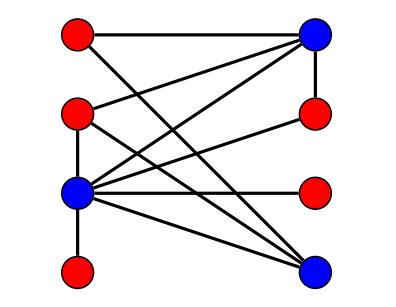
\includegraphics[keepaspectratio,alt={Independent set and Vertex cover example graph}]{independent_set_vertex_cover.png}}
\caption{Independent set and Vertex cover example graph}
\end{figure}

In this example graph:

\begin{itemize}
\tightlist
\item
  there is an independent set of size 5 (the red vertices)
\item
  there is a vertex cover of size 3 (the blue vertices)
\end{itemize}

For a graph \(G\) with \(n\) vertices:

\begin{itemize}
\tightlist
\item
  \(G\) has an independent set of size \(k\) if and only if \(G\) has a
  vertex cover of size \(n - k\)
\end{itemize}

Therefore, the independent set and vertex cover decision problems are
polynomial-time equivalent (they can be transformed into each other in
polynomial time via the above relationship).

    \subsection{Clique}\label{clique}

The clique problem is defined as:

\begin{itemize}
\tightlist
\item
  Given a graph \(G=(V,E)\) and an integer \(k\),
\item
  does \(G\) contain a clique of size at least \(k\)?
\end{itemize}

A clique is a set of vertices in which every pair of distinct vertices
is connected by an edge.

The complement of a graph \(G=(V,E)\), denoted \(\overline{G}\), is the
graph with:

\begin{itemize}
\tightlist
\item
  the same vertex set \(V\)
\item
  an edge between two vertices \(u\) and \(v\) in \(G\) if and only if
  \((u,v) \not\in E\)
\end{itemize}

A graph \(G\) has an independent set of size \(k\) if and only if its
complement \(\overline{G}\) has a clique of size \(k\).

Therefore, the Clique problem and the Independent Set problem are
polynomial-time equivalent, since one can be transformed into the other
via taking graph complements in polynomial time.

    \section{\texorpdfstring{The complexity class
\textbf{P}}{The complexity class P}}\label{the-complexity-class-p}

\subsection{Time complexity}\label{time-complexity}

For any function \(f\), , a decidable language \(L\) has time complexity
\(O(f)\) if there exist:

\begin{itemize}
\tightlist
\item
  a deterministic Turing machine \(T\) that decides \(L\), and
\item
  constants \(c>0\) and \(n_0 \geq 0\),
\end{itemize}

such that for every input \(x\) with \(|x| \geq n_0\),

\[
\text{Time}_T(X) \leq c \cdot f(|x|)
\]

Here:

\begin{itemize}
\tightlist
\item
  \(|x|\) denotes the length of the input,
\item
  \(Time_T(x)\) is the number of computation steps taken by \(T\) on
  input \(x\).
\end{itemize}

\subsection{Time complexity classes}\label{time-complexity-classes}

For a function \(f\), the complexity class \[
\text{TIME}(f)
\] (or sometimes \(\text{DTIME}(f)\), for deterministic time) is the set
of all languages \(L\) for which there exists a deterministic Turing
machine that decides \(L\) in \(O(f)\) time.

\subsection{\texorpdfstring{The class
\textbf{P}}{The class P}}\label{the-class-p}

The complexity class \textbf{P} is defined by:

\[
\textbf{P} = \bigcup_{k \geq 0} \text{TIME}[n^k]
\]

This is the class of all languages that can be decided in polynomial
time by a deterministic Turing machine.

The class \textbf{P} is commonly considered a mathematical model of
tractable (efficiently solvable) problems.

However, the correspondence with ``practical efficiency'' is only
approximate:

\begin{itemize}
\tightlist
\item
  A polynomial-time algorithm with a large exponent may still be
  impractical for real input sizes
\item
  The hidden constant factors in the \(O()\) notation may also be very
  large and dominate runtime in practice
\end{itemize}

Generally for naturally occurring problems in computer science, the
degree and constants are not too large.

    \subsubsection{Different models of
computation}\label{different-models-of-computation}

\begin{itemize}
\tightlist
\item
  A \(k\)-tape Turing machine that runs in \(t\) steps can be simulated
  by an equivalent single-tape Turing machine in \(O(t^2)\) time.
\item
  A single-tape Turing machine running in \(t\) steps can be simulated
  by a k-tape Turing machine in \(O(t)\) time.
\end{itemize}

Therefore, the complexity class \textbf{P} is invariant under these
standard models of computation (up to polynomial factors), including
single-tape, multi-tape, and other reasonable deterministic machine
models.

\subsubsection{Encodings}\label{encodings}

For any integer \(n\), the length of its representation in base \(b_1\)
base \(b_2\) differ by at most a constant factor, provided
\(b_1, b_2 \geq 2\).

For any graph \(G\), the length of the encoding of \(G\):

\begin{itemize}
\tightlist
\item
  as an adjacency matrix, and
\item
  as a list of edges
\end{itemize}

differ in size by at most a polynomial factor in the number of vertices.

Hence the class \textbf{P} is invariant under these reasonable encodings
of inputs (up to polynomial transformations of input length).

    \subsection{\texorpdfstring{Proving a problem is in
\textbf{P}}{Proving a problem is in P}}\label{proving-a-problem-is-in-p}

The class \textbf{P} is considered robust:

\begin{itemize}
\tightlist
\item
  it is invariant under reasonable choices of computational model
  (e.g.~single-tape vs multi-tape Turing machines)
\item
  it is also invariant under reasonable encodings of inputs
\end{itemize}

Therefore, when proving that a problem is in \textbf{P}, the exact
machine model or low-level encoding details are usually not important.

To show that a problem (language) is in \textbf{P}, the standard
approach is:

\begin{itemize}
\tightlist
\item
  Provide a deterministic algorithm that solves the problem in
  polynomial time
\end{itemize}

This algorithm can be described at a high level (e.g.~in pseudo-code),
as long as its correctness and polynomial running time can be justified:

\begin{itemize}
\tightlist
\item
  even a straightforward polynomial-time algorithm is useful, because it
  establishes that the problem is efficiently solvable in theory
\item
  however, finding such an algorithm often requires identifying a
  strategy that is significantly better than brute-force search
\end{itemize}

    \subsection{CNF}\label{cnf}

Many important computational problems involve logical formulas over
Boolean variables.

A Boolean formula \(f\) is in conjunctive normal form (CNF) if it can be
written as: \[
f = C_1 \land \ldots \land C_m
\] where each \(C_i\) is a clause.

A clause is a disjunction (OR) of literals: \[
C_i = L_{i1} \lor \ldots \lor L_{ik}
\]

A literal is either: - a variable, e.g., \(x\) - or its negation,. e.g.,
\(\neg x\)

A formula is in \(k\)-CNF if every clause contains at most \(k\)
literals.

    \subsubsection{Satisfiability}\label{satisfiability}

A Boolean formula \(f\) in CNF is satisfiable f there exists an
assignment of TRUE / FALSE values to its variables such that the formula
evaluates to TRUE.

\begin{itemize}
\tightlist
\item
  \(f\) is TRUE iff all clauses are TRUE
\item
  a clause is TRUE iff at least one of its literals is TRUE
\end{itemize}

\paragraph{The Satisfiability problem}\label{the-satisfiability-problem}

The Satisfiability problem (SAT) is:

\begin{quote}
Given a CNF formula \(f\), does there exist a truth assignment to its
variables such that \(f\) evaluates to TRUE?
\end{quote}

\paragraph{\texorpdfstring{\(k\)-Satisfiability
problem}{k-Satisfiability problem}}\label{k-satisfiability-problem}

A restricted version is the \(k\)-SAT problem:

\begin{quote}
Given a CNF formula in which every clause has at most \(k\) literals, is
the formula satisfiable?
\end{quote}

    \paragraph{2-Satisfiability}\label{satisfiability}

2-Satisfiability is in \textbf{P}.

The proof is as follows:

\begin{enumerate}
\def\labelenumi{\arabic{enumi}.}
\setcounter{enumi}{-1}
\tightlist
\item
  Declare:

  \begin{itemize}
  \tightlist
  \item
    all clauses unsatisfied
  \item
    all literals unassigned
  \end{itemize}
\item
  Select an arbitrary unassigned variable \(x\). Assign:

  \begin{itemize}
  \tightlist
  \item
    \(x =\) TRUE
  \item
    \$\neg x \$ = FALSE
  \end{itemize}
\item
  Select an unsatisfied clause \(I_i \lor I_j\):

  \begin{itemize}
  \tightlist
  \item
    if both literals are unassigned:

    \begin{itemize}
    \tightlist
    \item
      ignore the clause
    \end{itemize}
  \item
    if at least one literal is assigned TRUE:

    \begin{itemize}
    \tightlist
    \item
      declare the clause satisfied
    \end{itemize}
  \item
    if one literal is FALSE and the other is unassigned:

    \begin{itemize}
    \tightlist
    \item
      assign the unassigned literal to TRUE
    \item
      assign its negation to FALSE
    \item
      mark the clause as satisfied
    \end{itemize}
  \item
    if both literals are FALSE:

    \begin{itemize}
    \tightlist
    \item
      restart the algorithm
    \item
      set \(x =\) FALSE and \(\neg x =\) TRUE
    \item
      if the same conflict occurs again after this restart, declare the
      formula unsatisfiable
    \end{itemize}
  \end{itemize}
\item
  Repeat step 2 until either:

  \begin{itemize}
  \tightlist
  \item
    all clauses are satisfied:

    \begin{itemize}
    \tightlist
    \item
      return satisfiable
    \end{itemize}
  \item
    remaining unsatisfied clauses contain only unassigned variables:

    \begin{itemize}
    \tightlist
    \item
      return to step 1
    \end{itemize}
  \end{itemize}
\end{enumerate}

    \subsection{Polynomial-time reduction}\label{polynomial-time-reduction}

An alternative way to prove that a problem is in \textbf{P} is by using
a reduction.

Informally, a problem P is reducible to a problem Q if an algorithm for
solving Q can be used as a subroutine to solve P.

Formally: a language \(L_1\) is polynomially reducible to \(L_2\),
denoted \[ L_1 \leq L_2 \] if there exists a function \(f\) such that:

\begin{itemize}
\tightlist
\item
  \(f\) is computable in polynomial time, and
\item
  for all inputs \(x\):
\end{itemize}

\[x \in L_1 \iff f(x) \in L_2\]

The function \(f\) transforms instances of problem \(L_1\) into
instances of problem \(L_2\) such that:

\begin{itemize}
\tightlist
\item
  YES-instances stay YES-instances
\item
  NO-instances stay NO-instances
\end{itemize}

So solving \(L_2\) automatically gives a way to solve \(L_1\).

The key property of this is that:

\begin{itemize}
\tightlist
\item
  if \$L\_1 \leq L\_2 \$ and \(L_2 \in \mathbf{P}\), then
  \(L_1 \in \mathbf{P}\)
\end{itemize}

    \subsubsection{\texorpdfstring{\(k\)-colourability}{k-colourability}}\label{k-colourability}

A (vertex) colouring of a graph \(G = (V,E)\) is a function: \[
f: V \to {1, \ldots,k}
\]

A colouring is proper if for every edge \((u,v) \in E\), \[
f(u) \neq f(v)
\]

That is, adjacent vertices must receive different colours.

The \(k\)-Colourability problem is:

\begin{quote}
Given a graph G, does there exist a proper colouring of G using at most
\(k\) colours?
\end{quote}

Note that when \(k = 2\), this problem becomes exactly the bipartite
graph problem.

\begin{quote}
Given a graph G, can the vertices be split into two disjoint sets, such
that no vertex shares an edge with any other vertex in its set?
\end{quote}

\subsubsection{Reducing 2-Colourability to
2-Satisfiability}\label{reducing-2-colourability-to-2-satisfiability}

The 2-Colourability (bipartite) problem can be reduced to 2-SAT:

\begin{itemize}
\tightlist
\item
  for each vertex \(v_i\) of the graph

  \begin{itemize}
  \tightlist
  \item
    create a variable \(x_i\)
  \end{itemize}
\item
  for each edge \((v_i, v_j)\):

  \begin{itemize}
  \tightlist
  \item
    add two clauses:

    \begin{itemize}
    \tightlist
    \item
      \((x_i \lor x_j)\)
    \item
      \((\neg x_i \lor \neg x_j)\)
    \end{itemize}
  \end{itemize}
\end{itemize}

This converts the 2-Colourability problem to the 2-Satisfiability
problem in \(O(V+E)\).

Solving the 2-Colourability problem can now be done by solving the
equivalent 2-Satisfiability problem:

\begin{itemize}
\tightlist
\item
  if the formula is satisfiable, define the 2-colouring by setting TRUE
  variables to colour 1 and FALSE to colour 2
\item
  if two adjacent vertices get the same colour, then the corresponding
  edge clauses are not satisfied (contradiction)
\item
  thus we obtain a proper 2-colouring
\end{itemize}

    \section{The complexity class NP}\label{the-complexity-class-np}

\subsection{Certificate}\label{certificate}

A certificate (or witness) is a string that provides evidence that an
input belongs to a language.

More formally, for a language \(L\), a certificate for an input \(x\) is
a string \(c\) that can be used by a polynomial-time verification
algorithm to confirm that:

\[ x \in L \]

\begin{itemize}
\tightlist
\item
  A certificate is often thought of as a proposed solution that can be
  checked efficiently.
\item
  For inputs whose answer is YES, there exists a certificate that
  verifies this.
\item
  For inputs whose answer is NO, no valid certificate exists.
\end{itemize}

For example:

\begin{itemize}
\tightlist
\item
  Satisfiability (SAT):

  \begin{itemize}
  \tightlist
  \item
    a certificate is a satisfying assignment of truth values to the
    variables
  \end{itemize}
\item
  \(k\)-Colourability:

  \begin{itemize}
  \tightlist
  \item
    a certificate is a proper \(k\)-colouring of the graph
  \end{itemize}
\item
  Hamiltonian Cycle:

  \begin{itemize}
  \tightlist
  \item
    a certificate is a Hamiltonian cycle in the graph
  \end{itemize}
\end{itemize}

    \subsection{Verifiers}\label{verifiers}

An acceptor machine V that halts on all inputs is called a verifier for
a language \(L\) if

\[
L = {w \mid V \text{ accepts \langle w,c\rangle  for some string c}}
\]

\begin{itemize}
\tightlist
\item
  the string c is called a certificate (or witness) for w
\item
  the verifier receives both the input w and the certificate c
\item
  if \(w \in L\), then there exists a certificate c that causes V to
  accept
\item
  If \(w \not\in L\), then no certificate causes V to accept
\end{itemize}

A verifier is said to be polynomial-time if:

\begin{itemize}
\tightlist
\item
  V runs in polynomial time with respect to the size of its input, and
\item
  there exists a polynomial \(p\) such that, for every \(w \in L\),
  there is a certificate c satisfying
\end{itemize}

\[
|c| \leq p(|w|)
\]

That is, every YES-instance has a certificate whose length is polynomial
in the size of the input.

    \subsection{\texorpdfstring{The class
\textbf{NP}}{The class NP}}\label{the-class-np}

The class \textbf{NP} is the set of all languages that have a
polynomial-time verifier.

That is, a language is in \textbf{NP} if every YES-instance has a
polynomial-size certificate that can be verified in polynomial time.

Examples of problems in \textbf{NP} include:

\textbf{Composite Number} \textgreater{} Given a positive integer \(k\),
are there integers \(u, v > 1\) such that \(u \cdot v = k\)

\begin{itemize}
\tightlist
\item
  A certificate is the pair \((u,v)\).
\item
  Verification consists of checking that:

  \begin{itemize}
  \tightlist
  \item
    \(u,v>1\), and
  \item
    \(u \cdot v=k\)
  \end{itemize}
\item
  Both checks can be performed in polynomial time.
\end{itemize}

\textbf{Subset Sum} \textgreater{} Given a collection of positive
integers \(S = {a_1, \ldots, a_k}\) and a target integer \(t\), is there
a subset T \subseteq S whose elements sum to \(t\)?

\begin{itemize}
\tightlist
\item
  A certificate is the subset T.
\item
  Verification consists of summing the elements of T and checking
  whether the result is \(t\).
\item
  This can be done in polynomial time.
\end{itemize}

Some problems that are probably not in \textbf{NP} include:

\textbf{No Hamiltonian Cycle} \textgreater{} Given a graph G, is it true
that g has no Hamiltonian cycle?

\begin{itemize}
\tightlist
\item
  a Hamiltonian cycle itself is a certificate that a graph does have a
  Hamiltonian cycle
\item
  However, it is not known how to provide a polynomial-size certificate
  that proves a graph has no Hamiltonian cycle.
\end{itemize}

    \subsection{Non-deterministic
machines}\label{non-deterministic-machines}

An alternative definition of the class \textbf{NP} is given using
non-deterministic Turing machines.

A non-deterministic Turing machine NT can be viewed as a computation
tree:

\begin{itemize}
\tightlist
\item
  \[NT(x)\] denotes the tree of all possible computation paths on input
  \(x\)
\item
  Each node is a configuration, and each branch represents a possible
  nondeterministic choice
\item
  \(NT\) accepts \(x\) if at least one computation path ends in an
  accept state
\end{itemize}

\subsubsection{Non-deterministic TM time
complexity}\label{non-deterministic-tm-time-complexity}

Let NT be a non-deterministic Turing machine.

The time complexity of NT on input \(x\), denoted:

\[
\text{NTime}_{NT}(x)
\]

is defined as the number of steps in the shortest accepting path of
\(NT(x)\) if there is one, otherwise it is the number of steps in the
shortest rejecting path.

If not all paths of \(NT(x)\) halt, then \(\text{NTime}_{NT}(x)\) is
undefined.

For a function \(f\), we say a language \(L\) is decidable in
non-deterministic time \(O(f)\) if

\begin{itemize}
\tightlist
\item
  there exists a non-deterministic Turing machine NT such that:

  \begin{itemize}
  \tightlist
  \item
    NT decides \(L\)
  \item
    and there exist constants \(c>0\), \(n_0\) such that for all inputs
    \(x\) with \(|x|>n\), every computation path of \(NT(x)\) halts
    within:
  \end{itemize}
\end{itemize}

\[
\text{NTime}_{NT} (x) \leq c \cdot f(|x|)
\]

\subsubsection{The class NTIME(f)}\label{the-class-ntimef}

The class \[
\text{NTIME}(f)
\] is the set of all languages that can be decided by a nondeterministic
Turing machine in time \(O(f)\).

\subsection{Alternative definition of
NP}\label{alternative-definition-of-np}

Using non-deterministic machines, \textbf{NP} can be defined as:

\[
\mathbf{NP} = \bigcup_{k \geq 0} \text{NTIME}[n^k]
\]

This is the class of all languages that can be decided by a
nondeterministic Turing machine in polynomial time.

    \subsection{\texorpdfstring{\textbf{P} =
\textbf{NP}}{P = NP}}\label{p-np}

The question of whether \textbf{P = NP} is one of the most important
open problems in computer science.

It asks whether every problem whose solution can be verified efficiently
can also be solved efficiently.

Equivalently, does the existence of a short (polynomial-size)
certificate guarantee the existence of a polynomial-time algorithm to
find such a certificate?

    \subsection{Complete problems}\label{complete-problems}

Any complexity class can be structured using polynomial-time reductions.

\begin{itemize}
\tightlist
\item
  We say \(L_1\) is related to \(L_2\) if \(L_1 \leq L_2\)
\item
  This induces a notion of relative difficulty between problems
\end{itemize}

This allows us to group problems into equivalence classes:

\begin{itemize}
\tightlist
\item
  Two problems are in the same equivalence class if they are
  polynomial-time reducible to each other
\end{itemize}

\[
L_1 \leq L_2 \text{ and } L_2 \leq L_1
\]

\begin{itemize}
\tightlist
\item
  Such problems are considered equally hard (up to polynomial time)
\end{itemize}

\subsubsection{Ordering by reduction}\label{ordering-by-reduction}

Polynomial-time reductions define a preorder on problems:

\begin{itemize}
\tightlist
\item
  if \(L_1 \leq L_2\), then \(L_1\) is no harder than \(L_2\)
\end{itemize}

This induces a partial ordering on equivalence classes of problems.

\subsubsection{Complete problems}\label{complete-problems-1}

A problem \(L\) in a complexity class \(C\) is called complete for \(C\)
if:

\begin{itemize}
\tightlist
\item
  \(L \in C\), and
\item
  every problem in \(C\) reduces to \(L\) in polynomial time
\end{itemize}

\[
\forall L' \in C, \quad L' \leq L
\]

Complete problems are the hardest problems in the class (up to
polynomial-time reductions): - If we can solve one complete problem
efficiently, then we can solve all problems in the class efficiently

    \subsection{NP-completeness}\label{np-completeness}

NP-complete problems are the hardest problems in NP.

They have the property that:

\begin{itemize}
\tightlist
\item
  they are in NP, and
\item
  every problem in NP can be reduced to them in polynomial time
\end{itemize}

This means:

\begin{itemize}
\tightlist
\item
  If any NP-complete problem can be solved in polynomial time, then
  every problem in NP can be solved in polynomial time.
\end{itemize}

To show that \(L\) is NP-complete, it must be shown that every language
in \(NP\) can be reduced to \(L\) in polynomial time:

\begin{itemize}
\tightlist
\item
  once one NP-complete language \(L_0\) is know, any language \(L\) can
  be shown to be NP-complete by showing that \(L_0 \leq L\) and
  \(L \in NP\).
\end{itemize}

    \subsubsection{NP-completeness of
Satisfiability}\label{np-completeness-of-satisfiability}

The Cook-Levin theorem is that \textgreater{} Satisfiability is
NP-complete

so:

\begin{itemize}
\tightlist
\item
  SAT is in NP, and
\item
  every problem in NP can be reduced to SAT in polynomial time
\end{itemize}

This would mean that:

\begin{itemize}
\tightlist
\item
  \textbf{P} = \textbf{NP} if and only if Satisfiability is in
  \textbf{P}.
\end{itemize}

    \subsection{Ladner's theorem}\label{ladners-theorem}

Ladner's theorem states that:

\begin{itemize}
\tightlist
\item
  if \textbf{P} \(\neq\) \textbf{NP}, then there exist problems in NP
  that are neither in P nor NP-complete.
\end{itemize}

Such problems are called NP-intermediate problems.

This means that, if \textbf{P} \(\neq\) \textbf{NP}, then:

\begin{itemize}
\tightlist
\item
  \textbf{NP} is strictly larger than \textbf{P}
\item
  not all problems in \textbf{NP} \(\setminus\) \textbf{P} are
  NP-complete
\item
  there exist middle problems of intermediate difficulty
\end{itemize}

    \subsection{NP-intermediate
candidates}\label{np-intermediate-candidates}

Proving that a problem is NP-intermediate would imply that \textbf{P}
\(\neq\) \textbf{NP}. Therefore, no problem has been proven to be
NP-intermediate.

However, there are several candidates that are believed to lie in
NP-intermediate.

A leading candidate is:

\textbf{Graph Isomorphism}

\begin{quote}
Given two graphs \(G = (V_G, E_G)\) and \(H = (V_H, E_H)\), are G and H
isomorphic?
\end{quote}

Two graphs are isomorphic if there is a bijection

\[f: V_G \to V_H \]

such that \[ 
(u,v) \in E_G \iff (f(u),f(v)) \in E_H
\]

    \subsection{NP-hard}\label{np-hard}

To prove a problem \(\Pi\) is \textbf{NP}-complete, two steps must be
performed:

\begin{enumerate}
\def\labelenumi{\arabic{enumi}.}
\tightlist
\item
  Show that \(\Pi \in\) \textbf{NP}
\item
  Find a known \textbf{NP}-complete problem \(\Pi'\) and show that
  \(\Pi' \leq \Pi\)
\end{enumerate}

If step 2 can be shown, but step 1 is not known or does not hold, then
\(\Pi\) is \textbf{NP}-hard.

    \subsection{Proving reducability}\label{proving-reducability}

There are three general methods to prove that a known NP-complete
problem \(\Pi'\) is polynomial-time reducible to a problem \(\Pi\):

\begin{itemize}
\tightlist
\item
  restriction

  \begin{itemize}
  \tightlist
  \item
    show that \(\Pi'\) is a special case (restriction/subproblem) of
    \(\Pi\)
  \item
    That is, every instance of \(\Pi'\) is also an instance of \(\Pi\)
  \end{itemize}
\item
  local replacement

  \begin{itemize}
  \tightlist
  \item
    show that every basic unit (e.g.~variable, clause, edge) in an
    instance of \(\Pi'\) can be replaced by a corresponding structure in
    \(\Pi\)
  \item
    the replacement must be uniform and preserve correctness
  \end{itemize}
\item
  component design

  \begin{itemize}
  \tightlist
  \item
    show that instances of \(\Pi\) can be used to construct gadgets
    (components) that simulate the behaviour of \(\Pi'\)
  \item
    these gadgets are then combined to encode any instance of \(\Pi'\)
  \end{itemize}
\end{itemize}

    \subsection{\texorpdfstring{\textbf{NP}-completeness of Vertex
Cover}{NP-completeness of Vertex Cover}}\label{np-completeness-of-vertex-cover}

Recall the vertex cover problem:

\begin{quote}
Given a graph \(G=(V,E)\) and an integer \(k\), does \(G\) contain a
vertex cover of size at most \(k\)?
\end{quote}

A vertex cover is a set of vertices such that every edge in the graph
has at least one endpoint in the set.

This problem is in \textbf{NP}:

\begin{itemize}
\tightlist
\item
  a certificate is a proposed vertex cover
\end{itemize}

To show that Vertex Cover is NP-complete, Satisfiability (known to be
\textbf{NP}-complete) can be reduced to Vertex Cover:

Given a CNF formula \(f\) with \(n\) variables and clauses
\(C_1, C_2, \ldots, C_m\):

\begin{itemize}
\tightlist
\item
  for each variable \(x\):

  \begin{itemize}
  \tightlist
  \item
    create two adjacent vertices \(x^t\) and \(x^f\)
  \item
    these represent the literals \(x\) and \(\neg x\)
  \end{itemize}
\item
  for each clause \(C_j\) of size \(n_j\):

  \begin{itemize}
  \tightlist
  \item
    create a complete graph (clique) \(G_j\) on \(n_j\) vertices
  \item
    each vertex corresponds to one literal in the clause
  \end{itemize}
\item
  for each literal vertex in a clause gadget:

  \begin{itemize}
  \tightlist
  \item
    connect it to the corresponding literal vertex in the variable
    gadget
  \end{itemize}
\item
  set \(k = n + \sum_{j=1}^m (n_j - 1)\)
\end{itemize}

This construction can be carried out in polynomial time.

\begin{figure}
\centering
\pandocbounded{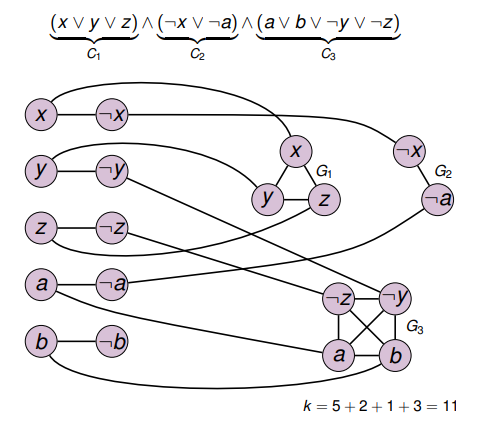
\includegraphics[keepaspectratio,alt={SAT to Vertex Cover}]{sat_vc.png}}
\caption{SAT to Vertex Cover}
\end{figure}

Then, exists a truth assignment that satisfies the formula \(f\) if and
only if there exists a vertex cover of the constructed graph with size
at most \(k\).

Therefore, since SAT is NP-complete, it follows that vertex cover is
NP-complete.

    \subsection{NP-completeness of Clique}\label{np-completeness-of-clique}

Recall the clique problem:

\begin{quote}
Given a finite graph \(G\) and an integer \(k\), does \(G\) have a
clique of size \(k\)?
\end{quote}

A clique is a set of vertices such that every pair of distinct vertices
in the set is connected by an edge.

There is a straightforward reduction from Vertex Cover to Clique:

Let \(\overline{G}\) denote the complement of \(G\), i.e.~the graph
obtained by:

\begin{itemize}
\tightlist
\item
  keeping the same vertices, and
\item
  replacing every non-edge of \(G\) with an edge, and vice versa
\end{itemize}

Then:

\begin{itemize}
\tightlist
\item
  A set of vertices \(W\) is a vertex cover in \(G\) if and only if
  \(V \setminus W\) is a clique in \(\overline{G}\).
\end{itemize}

    \subsection{\texorpdfstring{\textbf{NP}-completeness of Hitting
Set}{NP-completeness of Hitting Set}}\label{np-completeness-of-hitting-set}

The Hitting Set problem is as follows:

\begin{quote}
Given a collection \(C\) of subsets of a set \(S\) and a positive
integer \(k\), does there exist a hitting set for \(C\) of size at most
\(k\)?
\end{quote}

A hitting set is a subset \(S' \subseteq S\) such that \(S'\) contains
at least one element from each subset from \(C\).

Hitting Set is in \textbf{NP}:

\begin{itemize}
\tightlist
\item
  the subset \(S'\) is the certificate
\item
  it can be verified in polynomially time if \(S'\) contains an element
  from each subset in \(C\)
\end{itemize}

To show that Hitting Set is \textbf{NP}-complete:

\begin{itemize}
\tightlist
\item
  restrict it to instance with \(|c| = 2\) for all \(c \in C\)
\item
  i.e., every set \(c\) in \(C\) has 2 elements
\end{itemize}

Then this restricted problem is equivalent to Vertex Cover:

\begin{itemize}
\tightlist
\item
  let \(S\) be the set of vertices of a graph \(G\)
\item
  let each subset \(c \in C\) correspond to an edge of G

  \begin{itemize}
  \tightlist
  \item
    if an edge joins vertices \(u\) and \(v\), then the corresponding
    subset is \({u,v}\)
  \end{itemize}
\end{itemize}

A hitting set \(S'\) must contain at least one element from every subset
in \(C\).

Equivalently:

\begin{itemize}
\tightlist
\item
  \(S'\) must contain at least one endpoint of every edge in \(G\)
\end{itemize}

which is exactly the definition of a vertex cover.

Therefore:

\begin{itemize}
\tightlist
\item
  Vertex Cover \(\leq\) Hitting Set
\end{itemize}

    \subsubsection{\texorpdfstring{\textbf{NP}-completeness of
3-SAT}{NP-completeness of 3-SAT}}\label{np-completeness-of-3-sat}

To show that 3-SAT is NP-complete, SAT can be reduced to 3-SAT:

Replace every clause \[ C = x_1 \lor x_2 \lor \ldots \lor x_k \] with
\(k > 3\) by:

\[ 
C' = (x_1 \lor x_2 \lor y_1) \land (\neg y_1 \lor x_3 \lor y_2) \land \ldots \land (\neg y_{k-3} \lor x_{k-1} \lor x_k) 
\]

\(C\) is satisfiable if and only if \(C'\) is, since at least one of the
literals other than the \(y\)'s must be TRUE.

    \subsection{Reducing SAT to Clique}\label{reducing-sat-to-clique}

Another way to show that Clique is \textbf{NP}-complete is to reduce SAT
to Clique.

Given a CNF formula \(f\) with clauses \(C_1, C_2, \ldots, C_k\):

\begin{itemize}
\tightlist
\item
  for each literal \(x\) in clause \(C_j\), create a vertex

  \begin{itemize}
  \tightlist
  \item
    each vertex represents a specific occurrence of a literal in a
    clause
  \end{itemize}
\item
  add an edge between two vertices if:

  \begin{itemize}
  \tightlist
  \item
    they come from different clauses, and
  \item
    they are not contradictory literals (i.e.~not \(x\) and \(\neg x\))
  \end{itemize}
\end{itemize}

A clique of size k corresponds to choosing:

\begin{itemize}
\tightlist
\item
  exactly one literal from each clause
\item
  such that all chosen literals are mutually consistent
\end{itemize}

\begin{figure}
\centering
\pandocbounded{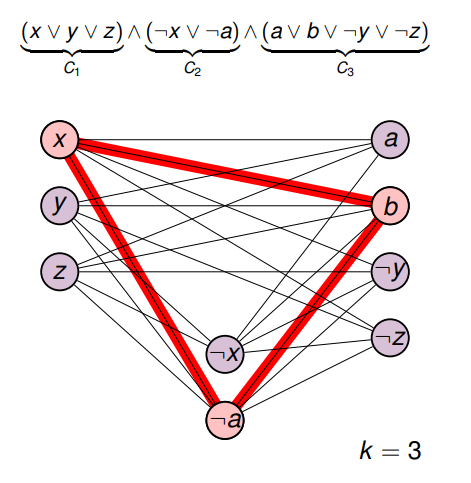
\includegraphics[keepaspectratio,alt={SAT to Clique}]{sat_clique.png}}
\caption{SAT to Clique}
\end{figure}


    % Add a bibliography block to the postdoc
    
    
    
\end{document}
